\begin{displayquote}
  % hack to stop the displayquote from eating the [
  {[}\dejafu{} is] A martial art in which the user's limbs move in
  time as well as space, [\ldots] It is best described as ``the
  feeling that you have been kicked in the head this way
  before.'' \parencite{pratchett2001}
\end{displayquote}

\noindent
Specialised tools are necessary to test concurrent programs.  In this
chapter we present and evaluate \dejafu{}, our library for testing
concurrency in Haskell.  We give an overview of the
tool~\sref{dejafu-whatis}, including the scope of bugs we aim to
detect, and present our abstraction over the GHC Haskell concurrency
functionality~\sref{dejafu-monadconc}.  We then show an example of a
small logic puzzle which we can represent as a concurrent
program~\sref{dejafu-100}.  We explain how programs using our
abstraction are executed~\sref{dejafu-execution}, and give our
semantic rules~\sref{dejafu-semantics}.  We explain how we test
programs~\sref{dejafu-testing} and how we present execution traces to
the user~\sref{dejafu-traces}.  We then argue the correctness of our
approach~\sref{dejafu-correctness}.  We present three case
studies~\sref{dejafu-casestudies}, and finally evaluate our
results~\sref{dejafu-evaluation}.

This chapter is derived from our previous work \cite{walker2015} and
\cite{YCS-2016-503}.

\section{What is \dejafu{}?}
\label{sec:dejafu-whatis}

\dejafu{} is a tool for testing concurrent Haskell programs.  It works
by providing a typeclass abstraction over the concurrency operations
of interest, called \verb|MonadConc|, and using an implementation of
this class based on inspectable continuations to explore the
nondeterministic behaviours of a program under test.

\begin{listing}
\centering
\begin{cminted}{haskell}
runSCTWithSettings :: MonadConc m
  => Settings m a
  -> ConcT m a
  -> m [(Either Failure a, Trace)]
\end{cminted}
\caption{The core API of \dejafu{}.}\label{lst:dejafucore}
\end{listing}

\Cref{lst:dejafucore} gives the type signature of the function at the
heart of \dejafu{}.  The first parameter is configuration, controlling
how \dejafu{} explores the space of executions.  The second is the
concurrent program to test: \verb|ConcT m| is \dejafu{}'s
implementation of \verb|MonadConc|, it is parameterised by some monad
\verb|m| which is used to provide mutable variables.  Typically this
\verb|m| will be \verb|IO|.  The function returns a collection of
tuples.

The outputs which \dejafu{} produces are pairs, where the first
component is the result of the program and the second is the execution
trace which led to it.  A program may not complete successfully: for
example, it may deadlock.  If the program does complete successfully,
the first component of the tuple will be a \verb|Right| containing the
actual value produced, otherwise it will be a \verb|Left| and the
\verb|Failure| value will show what went wrong.  A \verb|Trace| is a
list of scheduling decisions, with a summary of what the chosen thread
did in that step of execution.

In outline, \verb|runSCTWithSettings| works like so:

\begin{enumerate}
\item Repeat until there are no more executions:
  \begin{enumerate}
  \item Set up the initial state, where only the main thread exists
  \item While the main thread exists, and there are runnable threads:
    \begin{enumerate}
    \item Choose a thread
    \item Run the next action in that thread
    \end{enumerate}
  \item Add the result pair to the output
  \end{enumerate}
\end{enumerate}

We produce different schedules by making step (b) stateful.  \dejafu{}
supports three ways to explore the behaviours of a concurrent program:

\begin{description}
\item[Randomly] Threads are chosen using a uniform random
  distribution.  Exploration terminates after a fixed number of
  executions.

\item[Swarm] Threads are chosen using a weighted random distribution.
  Exploration terminates after a fixed number of executions.  We
  discuss this algorithm further in \Cref{chp:algorithms}.

\item[DPOR] Uses a notion of ``to-do sets,'' where each scheduling
  point has an associated set of threads to try in future executions.
  Execution terminates when all such sets are empty.

  During execution, at each scheduling point, if the previously chosen
  thread is still runnable, choose that; otherwise, take all runnable
  threads, choose one arbitrarily, and record the others in the to-do
  set for this scheduling point.

  After execution, the trace is examined to find pairs of dependent
  actions: for each thread $T$, for each action in thread $T$, find
  the most recent dependent action (if one exists) in a different
  thread, and add $T$ to the to-do set corresponding to that
  scheduling point if $T$ is runnable; otherwise add all runnable
  threads.

  There are some subtleties and additional optimisations, which we
  discuss further in \Cref{sec:dejafu-testing}.
\end{description}

\subsection{What sort of bugs can \dejafu{} detect?}
\label{sec:dejafu-whatis-bugs}

\dejafu{} produces a list of \verb|(Either Failure a, Trace)| values,
where the \verb|a| is the result of a successful execution.  \dejafu{}
supports ``online'' filtering, removing uninteresting result pairs or
execution traces as they are found.  Configuration for this online
filtering is passed to \verb|runSCTWithSettings| via the
\verb|Settings| value.  \dejafu{} tests use predicates on the final,
filtered, list of pairs: these predicates can check anything, for
example all results being \verb|Right|s and equal.  If an execution
yields a \verb|Left| value, we say that it has \emph{failed}.
\dejafu{} can detect two different types of failure:

\begin{description}
\item[Deadlocks] Every thread is blocked.
\item[Uncaught exceptions] The main thread is killed by an exception.
\end{description}

There are two types of failure which \dejafu{} itself may raise:

\begin{description}
\item[Aborts] All scheduling decisions are forbidden by schedule
  bounding.
\item[Internal errors] An internal invariant is broken.  This
  indicates a bug in \dejafu{}.
\end{description}

Finally, there are two types of failure which can arise through
improper use of \dejafu{}, due to weaknesses in the current API
design.

\begin{listing}
\centering
\begin{cminted}{haskell}
gives :: (Eq a, Show a) => [Either Failure a] -> Predicate a
gives expected = ProPredicate
    { pdiscard = \r  -> if r `elem` expected then Just DiscardTrace else Nothing
    , peval    = \xs -> go expected [] xs (defaultFail xs)
    }
  where
    go waitingFor alreadySeen ((x, _):xs) res
      -- If it's a result we're waiting for, move it to the
      -- @alreadySeen@ list and continue.
      | x `elem` waitingFor  = go (filter (/=x) waitingFor) (x:alreadySeen) xs res
      -- If it's a result we've already seen, continue.
      | x `elem` alreadySeen = go waitingFor alreadySeen xs res
      -- If it's not a result we expected, fail.
      | otherwise = res
    go [] _ [] res =
      res { _pass = True }
    go es _ [] res =
      res { _failureMsg = unlines (map (\e -> "Expected: " ++ show e) es) }

    defaultFail xs = Result
      { _pass       = False
      , _failures   = filter (\(r, _) -> r `notElem` expected) xs
      , _failureMsg = ""
      }
\end{cminted}
\caption[The \texttt{gives} predicate.]{The \texttt{gives} predicate.  The \texttt{pdiscard} component is used for online filtering, removing uninteresting traces as they are found.  The \texttt{peval} component takes the final list of pairs and determines if the test passes or fails.}\label{lst:gives}
\end{listing}

For an example of a \dejafu{} predicate, see \Cref{lst:gives}.  The
\verb|gives| predicate is used to check that a program produces
exactly the desired set of results, failing if unexpected results are
present or expected results are not.  The predicate reduces memory
usage by using online filtering to discard the execution traces of
expected results, as we are only interested in execution traces which
yield \emph{unexpected} results.  There is nothing special about
\verb|gives|, it is just a normal function written using the \dejafu{}
API.  It is provided as an example of the sort of thing that \dejafu{}
can be used to check.

\paragraph{Equivalence testing}
\dejafu{} supports testing the observational equivalence of two
concurrent programs.  Observational equivalence here means that the
observable effects of the program on a distinguished piece of shared
state, using some observation function provided by the programmer, are
equal for both programs.

\Cref{lst:evalSigWithSeed} shows the heart of the equivalence testing.
It is built on top of the usual \verb|runSCTWithSettings| function,
but encapsulates some concerns relevant to equivalence testing.  In
particular, \verb|evalSigWithSeed| introduces concurrent interference,
which is necessary to distinguish atomic from non-atomic operations in
some cases.  Every execution, including failing executions, yields an
observation value.  This is necessary because a failing execution may
nevertheless modify the state before it fails.  We build on top of
this function a tool to generate a number of initial states and
compare two programs for all of them.  Two programs are
observationally equivalent, up to the given interference and
observation functions, if each initial state yields the same sets
observations.

\begin{listing}
\centering
\begin{cminted}{haskell}
evalSigWithSeed :: (MonadConc m, Ord o)
  => (x -> ConcT m s)       -- ^ Create a new instance of the state.
  -> (s -> x -> ConcT m o)  -- ^ The observation to make.
  -> (s -> x -> ConcT m ()) -- ^ Perform some concurrent interference.
  -> (s -> ConcT m ())      -- ^ The expression to evaluate.
  -> x                      -- ^ Pure value used to initialise the state.
  -> m (Set (Maybe Failure, o))
\end{cminted}
\caption[The \texttt{evalSigWithSeed} function.]{The \texttt{evalSigWithSeed} function.  Runs a concurrent program and returns a set of observations and possible failures.}\label{lst:evalSigWithSeed}
\end{listing}

We build upon this further in \Cref{chp:coco} where we also discuss
refinement, and how to \emph{discover} rather than just \emph{test}
these properties.

\paragraph{Invariant testing}
A feature which \dejafu{} does \emph{not} currently have, but which
makes sense, is invariant testing.  A function could be provided to
register an arbitrary concurrency action as an invariant.  As
\dejafu{} drives the execution of the program under test, these
invariants can be checked atomically.  This would be similar to, but
more general than, the GHC Haskell function
\verb|always :: STM Bool -> STM ()|, which registers an invariant to
be checked at the end of STM transactions.

\subsection{Scope}
\label{sec:dejafu-whatis-scope}

We aim to support most of the functionality of GHC’s concurrency API.
However, some operations are more trouble than they're worth: for
example, operations which introduce additional sources of
nondeterminism, or which unavoidably require support from the runtime
system.  In particular, we do not support:

\begin{itemize}
\item Operations to block a thread until a file descriptor becomes
  available, as this introduces an additional source of
  nondeterminism.

\item Operations to query which capability (OS thread) a Haskell
  thread is running on, as this also introduces an additional source
  of nondeterminism.

\item Automatically detecting if a thread is deadlocked on an
  \verb|MVar| or \verb|TVar| and throwing an exception to it, as we
  cannot detect this situation in general without support from the
  garbage collector.
\end{itemize}

We also do not yet support \emph{bound threads}: a Haskell thread
which will always run on the same, unique, OS thread.  Bound threads
are essential for using the foreign function interface (FFI) to call C
libraries which use thread-local state, to ensure the Haskell thread
always sees its state and never the state of another thread.  We have
a prototype implementation, which is planned to be included in the
next major release of
\dejafu{}\footnote{\url{https://github.com/barrucadu/dejafu/issues/126}}.

\paragraph{Semantic departures}
In the functionality we do support, we model behaviour as close as
reasonably possible to GHC.  We make a few departures from the
traditional semantics where there is good reason to do so:

\begin{itemize}
\item Runtime errors, such as pattern match failures, can be caught as
  exceptions inside \verb|IO|.  As there is no non-\verb|IO| way to do
  the same, \dejafu{} cannot catch these errors.

\item We do not model threads delaying, and implement any delays as
  yields.  It is not clear how to incorporate time into the testing
  model.
\end{itemize}

\paragraph{Embedded \texttt{IO} actions}
\dejafu{} supports testing computations with embedded \verb|IO|
actions provided that the programmer ensures that the action is
atomic; that it is deterministic when executed with a fixed schedule;
and that it does not block on the action of another thread.  Failing
to meet any of these conditions may lead to incomplete testing.

\section{Abstracting over Concurrency}
\label{sec:dejafu-monadconc}

There are three ways of implementing a concurrency testing tool:
overriding the concurrency primitives of the language; instrumenting
the source program; or instrumenting the compiled program.  We adopt
the first approach in \dejafu{}.  Haskell's typeclass machinery lets
us specify an interface for concurrency, and to provide different
concrete implementations.  There is one implementation using the
\verb|IO| type and the standard functions; there is another using our
own type, which we can inspect.

\begin{listing}
\centering
\begin{cminted}{haskell}
class (Monad m, {- other constraints omitted -}) => MonadConc m where
  type MVar m :: * -> *
  -- other types omitted

  newEmptyMVar :: m (MVar m a)
  newEmptyMVar = newEmptyMVarN ""

  newEmptyMVarN :: String -> m (MVar m a)
  newEmptyMVarN _ = newEmptyMVar

  putMVar  :: MVar m a -> a -> m ()
  readMVar :: MVar m a -> m a
  takeMVar :: MVar m a -> m a
  -- other operations omitted
\end{cminted}
\caption{A fragment of the \texttt{MonadConc} typeclass.}\label{lst:monadconc}
\end{listing}

We call our typeclass \verb|MonadConc|: monads which do concurrency.
\Cref{lst:monadconc} shows a fragment.  To define an instance, the
programmer supplies concrete types for the abstract types and
implementations of all undefined operations.  Some operations have
default definitions: for example, there are two ways of constructing
an empty \verb|MVar|.  One way takes a name, which is displayed in
debugging information, the other does not.  Each has a default
definition in terms of the other, so the programmer must supply at
least one.

\begin{listing}
\centering
\begin{cminted}{haskell}
instance Monad n => MonadConc (ConcT m) where
  type MVar (ConcT m) = ModelMVar m
  -- other types omitted

  newEmptyMVarN n = toConc (ANewMVar n)

  putMVar  var a = toConc (\c -> APutMVar var a (c ()))
  readMVar var   = toConc (AReadMVar var)
  takeMVar var   = toConc (ATakeMVar var)
  -- other operations omitted
\end{cminted}
\caption{A fragment of the \texttt{MonadConc} testing implementation.}\label{lst:mvarops}
\end{listing}

\paragraph{Implementation}
The type for our testing implementation is called \verb|ConcT m|,
which is a monad that has access to mutable references provided by
some monad \verb|m|, which will typically be \verb|IO|.
\Cref{lst:mvarops} shows a fragment of the instance of
\verb|MonadConc| for this type.  Each concurrency operation is of the
same form: we take the arguments and wrap them up inside a data
structure whose final argument is a continuation, which is then
converted into a \verb|ConcT| value.

We represent a concurrent computation as a large value.  We can
inspect each step of the computation by looking at the data
constructor used.  We call these constructors \emph{primitive
  actions}.  With these actions we express the operations in the
\verb|MonadConc| class.

\section{The $n$ Prisoners Problem}
\label{sec:dejafu-100}

\begin{displayquote}
  There are $n$ prisoners in solitary cells.  There's a central living
  room with one light bulb.  No prisoner can see the light bulb from
  their own cell.  Every day, the warden picks a prisoner equally at
  random, and that prisoner visits the living room.  While there, the
  prisoner may toggle the bulb.  The prisoner also has the option of
  asserting that all $n$ prisoners have been to the living room.  If
  this assertion is false, all $n$ prisoners are shot.  However, if
  true, all prisoners are set free.  Thus, the assertion should only
  be made if the prisoner is 100\% certain of its validity.  The
  prisoners are allowed to get together one night in the courtyard, to
  discuss a plan.  What plan should they agree on, so that eventually,
  someone will make a correct assertion?
\end{displayquote}

We can express this puzzle as a concurrency problem: the warden is the
scheduler, each prisoner is a thread, and when the program terminates
every prisoner should have visited the living room.  So if every
thread (prisoner) is scheduled (taken to the room), the prisoners are
successful.  \dejafu{} can give us execution traces.  So, given some
way of setting up the prison, we can use \dejafu{} to execute it and
then examine the returned traces to discover if the prisoners are
successful.

\subsection{The Probabilistic Solution}

One school of thought says to just wait for $10 n$ days, because by
then it's unlikely that any prisoner has not visited the room.  The
chance that any one prisoner will have been consistently missed is
$\left(1 - \frac{1}{n}\right)^{10n}$, which converges to
$\frac{1}{e^{10}}$.

\Cref{lst:100good} shows an implementation of this strategy, and
\Cref{tbl:100rand} shows how the prisoners fare over 100 random
executions.  We see that the number of room visits grows a little
faster than ten for each additional prisoner, this is because of a
quirk of our implementation.  We have nominated one prisoner to be the
leader, who is the only prisoner able to declare that all have visited
the room.  So our implementation ends up waiting $10 (n - 1)$ days for
the non-leaders to visit, and then however many days it takes for the
leader to visit after that.

\begin{table}
  \centering
  \begin{tabular}{lrrrrrrrr} \toprule
    Prisoners          &   1 &   2    &   3    &   4    &   5    &   6    &   7    &   8 \\
    Successes          & 100 & 100    & 100    & 100    & 100    & 100    & 100    & 100 \\
    Failures           &   0 &   0    &   0    &   0    &   0    &   0    &   0    &   0 \\
    Avg.\@ Room Visits &   2 &  18.35 &  31.92 &  43.52 &  55.88 &  67.37 &  77.05 &  90.40 \\ \bottomrule
  \end{tabular}
  \caption{The behaviour of the probabilistic solution.}\label{tbl:100rand}
\end{table}

\subsection{The Perfect Solution}

Perhaps our prisoners are more cautious, and even a small chance of
death is too much.  They want to be certain of their success.  A slow
but simple strategy is for the prisoners, like in our probabiistic
solution, to nominate a leader.  Only the leader can declare to the
warden that everyone has visited the room.  Whenever a prisoner other
than the leader visits the room, if this is their first time in the
room with the light off, they turn it on, otherwise they do nothing.
Whenever the leader enters the room, they turn the light off.  When
the leader has turned the light off $n-1$ times, they tell the warden
that everyone has visited.  \Cref{lst:100perfect} shows an
implementation of these behaviours.

\begin{listing}
\begin{sublisting}{\textwidth}
\centering
\begin{cminted}{haskell}
leader :: MonadConc m => Int -> TVar (STM m) Int -> m ()
leader numPrisoners days = atomically $ do
  numDays <- readTVar days
  when (numDays < (numPrisoners - 1) * 10) retry

notLeader :: MonadConc m => TVar (STM m) Int -> m ()
notLeader days = forever $ atomically (modifyTVar days (+1))

prison :: MonadConc m => Int -> m ()
prison numPrisoners = do
  days <- atomically (newTVar 0)
  for_ [1..numPrisoners-1] (\_ -> fork (notLeader days))
  leader numPrisoners days
\end{cminted}
\caption{The probabilistic solution: just wait a long time and gamble.}\label{lst:100good}
\end{sublisting}

% [layout hack]: no gap between the listings otherwise
\vspace{1.5em}

\begin{sublisting}{\textwidth}
\centering
\begin{cminted}{haskell}
data Light = IsOn | IsOff

leader :: MonadConc m => Int -> TVar (STM m) Light -> m ()
leader numPrisoners light = go 0 where
  go counter = do
    counter' <- atomically $ do
      state <- readTVar light
      case state of
        IsOn -> do
          writeTVar light IsOff
          pure (counter + 1)
        IsOff -> retry
    when (counter' < prisoners - 1)
      (go counter')

notLeader :: MonadConc m => TVar (STM m) Light -> m ()
notLeader light = do
  atomically $ do
    state <- readTVar light
    case state of
      IsOn  -> retry
      IsOff -> writeTVar light IsOn
  forever yield

prison :: MonadConc m => Int -> m ()
prison numPrisoners = do
  light <- atomically (newTVar IsOff)
  for_ [1..numPrisoners-1] (\_ -> fork (notLeader light))
  leader numPrisoners light
\end{cminted}
\caption{The perfect solution: nominate a leader, who waits until they are certain that everyone has been in the room.}\label{lst:100perfect}
\end{sublisting}
\caption{Two solutions for the $n$ prisoners problem.}\label{lst:100sols}
\end{listing}

We can satisfy ourselves that this solution works for all cases by
using \dejafu{}'s systematic concurrency testing functionality, which
is a combination of dynamic partial-order reduction and schedule
bounding.  \Cref{tbl:100slow} shows how the number of schedules
explored and average number of room visits grows as the number of
prisoners increases.  It does not scale well.

This algorithm is something of a worst-case for DPOR.  Every thread is
modifying the same shared state, so DPOR has to try every
interleaving.  Taking another look at our prisoners, we can see two
things which a human would use to decide whether some schedules are
redundant or not:

\begin{table}
\begin{subtable}{\textwidth}
  \centering
  \begin{tabular}{lrrr} \toprule
    Prisoners          & 1 & 2 &    3 \\
    Schedules          & 1 & 5 & 2035 \\
    Avg.\@ Room Visits & 2 & 7 &  133 \\ \bottomrule
  \end{tabular}
  \caption{Using \dejafu{}'s default schedule bounds.}\label{tbl:100slow}
\end{subtable}

% [layout hack]: no gap between the tables otherwise
\vspace{1.5em}

\begin{subtable}{\textwidth}
  \centering
  \begin{tabular}{lrrrrrr} \toprule
    Prisoners          & 1 & 2 & 3   &  4   &    5 &      6 \\
    Schedules          & 1 & 1 & 4   & 48   & 1536 & 122880 \\
    Avg.\@ Room Visits & 2 & 4 & 7.5 & 11.5 &   16 &     21 \\ \bottomrule
  \end{tabular}
  \caption{Using a custom fair bound to prevent yields.}\label{tbl:100fast}
\end{subtable}
\caption{How the number of schedules grows with increasing prisoner numbers.}\label{tbl:100slowfast}
\end{table}

\begin{enumerate}
\item If we adopt any schedule other than alternating leader /
  non-leader, threads will block without doing anything.  So we should
  alternate.
\item When a non-leader has completed their task, they will always
  yield.  So we should never schedule a prisoner who will yield.
\end{enumerate}

\dejafu{} cannot make use of (1).  It would be possible to implement
this optimisation if \dejafu{} were able to compare values inside
\verb|TVar|s, as we would be able to check if any \verb|TVar| read
during a blocked transaction has a different value: if none do, the
transaction will just block again.  This would require a new primitive
action, as we cannot do that without putting an \verb|Eq| constraint
on \verb|writeTVar|.  We get part of the way there, though.  If a
thread is blocked in a transaction, \dejafu{} only tries executing it
again when at least one of the \verb|TVar|s it reads from has been
written to, which is similar to the version numbering scheme commonly
used in STM implementations \parencite{shavit1995}.

\dejafu{} can make use of (2).  \dejafu{} already bounds the maximum
number of times a thread can yield, so that it can test constructs
like spinlocks.  This is called \emph{fair bounding}.  The default
bound is five, but if we set it to zero \dejafu{} will never schedule
a thread which is going to yield.  \Cref{tbl:100fast} shows how the
number of schedules explored and average number of room visits grow
with this change.

This is better, but still scales poorly.  The program is still a bad
case for DPOR.  This is probably as good as we can do without adding
some extra primitives to \dejafu{} to optimise the case where we have
an \verb|Eq| instance available, or by using an alternative systematic
testing algorithm.  In \Cref{chp:algorithms} we will discuss an
alternative \emph{incomplete} approach to this, and other, concurrency
problems.

It's not the end for DPOR, however.  Empirical
studies \parencite{thomson2014} have found that many concurrency bugs can be
exhibited with only two or three threads.  Furthermore, most
real-world concurrent programs do not have every single thread
operating on the same bit of shared state.  So in practice, we will
tend not to see this exponential growth in schedules tried.

\section{Modelling Concurrent Programs}
\label{sec:dejafu-execution}

We represent operations in the \verb|MonadConc| typeclass by an
\verb|Action| type, which we give in full in
\Cref{sec:dejafu-semantics}.  Each action describes some effect and
contains a continuation.  A concurrent computation is a sequence of
these action values.  Each thread is terminated by a distinguished
\emph{stop} primitive, which has no continuation.  \Cref{lst:m} gives
the definition and typeclass instances of the \dejafu{} continuation
monad\footnote{\dejafu{} aims to support the latest three major
  releases of GHC, so in the real implementation we use conditional
  compilation.}.

\begin{listing}
\centering
\begin{cminted}{haskell}
newtype ConcT n a = M { runM :: (a -> Action n) -> Action n }

instance Functor (ConcT n) where
  fmap f m = M (\c -> runM m (c . f))

instance Applicative (ConcT n) where
  pure x  = M (\c -> AReturn (c x))
  f <*> v = M (\c -> runM f (\g -> runM v (c . g)))

instance Monad (ConcT n) where
  return  = pure
  m >>= k = M (\c -> runM m (\x -> runM (k x) c))

instance MonadFail (ConcT n) where
  fail e = M (\_ -> AThrow (MonadFailException e))
\end{cminted}
\caption{The \dejafu{} continuation monad.}\label{lst:m}
\end{listing}

\begin{listing}
\centering
\begin{cminted}{haskell}
pure id <*> v
  = M (\c -> AReturn (c id)) <*> v
  = M (\c -> runM (M (\c -> AReturn (c id))) (\g -> runM v (c . g)))
  = M (\c -> (\c -> AReturn (c id)) (\g -> runM v (c . g)))
  = M (\c -> AReturn ((\g -> runM v (c . g)) id))
  = M (\c -> AReturn (runM v (c . id)))
  = M (\c -> AReturn (runM v c))
 /= v
\end{cminted}
\caption{Expansion of the \texttt{Applicative} identity law.}\label{lst:areturn}
\end{listing}

\paragraph{Nonterminating executions}
\dejafu{} is only able to make scheduling decisions at the level of
primitive actions, which means that if evaluating a primitive action
does not terminate, \dejafu{} will hang.  As \Cref{lst:areturn} shows,
we deliberately break the \verb|Applicative| identity law, that
\verb|pure id <*> v = v| for all \verb|v|, to make some programs more
defined than they otherwise would be.

\begin{listing}
\centering
\begin{cminted}{haskell}
test = forever (pure "loop") where
  forever mx = mx >> forever mx
\end{cminted}
\caption{A simple non-terminating program.}\label{lst:forever}
\end{listing}

\Cref{lst:forever} shows a program which is made more defined by
breaking the law.  Neither \verb|>>| nor \verb|forever| correspond to
primitive actions, so they cannot be pre-empted.  If \verb|pure| did
not correspond to a primitive action either, then that expression
would cause \dejafu{} to loop forever as it tries to compute the
continuation.  This is an unhelpful result.  By breaking the laws and
introducing a way to interrupt the \verb|forever| computation,
\dejafu{} can instead report that trying to test this program exceeds
the execution length
limit\footnote{\url{https://github.com/barrucadu/dejafu/issues/27} and
  \url{issues/113}}.

\paragraph{Scheduling}
The choice of which thread to execute is made by a scheduler function.
The scheduler is called even if there is only one runnable thread, to
keep things simple.  A scheduler has the type declared in
\Cref{lst:scheduler}.  It is a stateful function which is given the
previous action and the runnable threads, which possibly returns a
thread to run.  If no thread is returned, the computation is aborted.
Aborting is used in the implementation of schedule bounding.  The
state is used in the implementation of DPOR and random scheduling: in
the former, the state is a list of scheduling decisions still to make;
in the latter, the state is a random number generator.

\begin{listing}
\centering
\begin{cminted}{haskell}
newtype Scheduler state = Scheduler
  { scheduleThread
    :: Maybe (ThreadId, ThreadAction)
    -> NonEmpty (ThreadId, Lookahead)
    -> state
    -> (Maybe ThreadId, state)
  }
\end{cminted}
\caption{The \dejafu{} \texttt{Scheduler} type.}\label{lst:scheduler}
\end{listing}

\paragraph{Success and failure}
When testing concurrent computations, we are interested in both
success and failure.  If a computation succeeds and returns a value,
we want to know that; if it enters a failure state such as deadlock,
we also want to know that.  As we have seen earlier, we achieve this
by reporting failure: the result of a single execution of the program
is a value of type \verb|(Either Failure result, Trace)|.

\subsection{Software Transactional Memory}

Transactions allow the atomic execution of a sequence of operations
involving \verb|TVar|s, transactional variables.  Unlike operations on
\verb|IORef|s or \verb|MVar|s, transactions are composable and the
whole remains atomic.  We express transactions in a similar way to
concurrent programs: as a monad of continuations over a primitive
action type.  As \dejafu{} drives the execution of a concurrent
program, it is possible to have arbitrarily complex effects which
appear atomic to the program under test.

A transaction evaluates to some success value, an uncaught exception,
or an abort.  If successful, it may also mutate some transactional
variables as a effect; otherwise it does not.  If it evaluates to an
uncaught exception, we raise the exception in the thread performing
the transaction.  If it evaluates to an abort, we block the thread
performing the transaction until at least one \verb|TVar| read in the
transaction is mutated by another thread.

\subsection{Relaxed Memory}

There are three memory models supported in \dejafu{}:

\begin{description}
\item[Sequential Consistency] This model is the most intuitive.  A program
  behaves as a simple interleaving of the actions in different threads.  When an
  \texttt{IORef} is written to, that write is immediately visible to all
  threads.

\item[Total Store Order (TSO)] Each thread has a write buffer.  A thread sees
  its writes immediately, but other threads will only see writes when they are
  \emph{committed}, which may happen later.  Writes by the same thread are
  committed in program order.

\item[Partial Store Order (PSO)] A relaxation of TSO where each thread
  has a write buffer for each \verb|IORef|.  Writes to different
  \verb|IORef|s by the same thread may not be committed in program
  order.
\end{description}

The default memory model for testing is TSO, as that most accurately
models the behaviour of modern x86 processors \parencite{owens2009}.  The
use of a relaxed memory model can require a much larger number of
schedules when \verb|IORef|s are shared between threads.

\paragraph{Write buffering}
We model relaxed memory by introducing buffers for thread writes.  When a thread
writes to an \verb|IORef|, the write is appended to its buffer.  When a thread
reads from an \verb|IORef|, it reads the value of the newest write in its buffer,
or the most recently committed value if the buffer is empty.  After a write is
committed, it is removed from its buffer.  Any non-empty buffer may have a write
committed, but only the oldest write in a buffer may be committed.  \Cref{fig:wb}
shows the arrangement of buffers for the three memory models in a system with
two threads and two \verb|IORef|s.

\begin{figure}
  \centering
  \begin{subfigure}{0.3\textwidth}
    \centering
    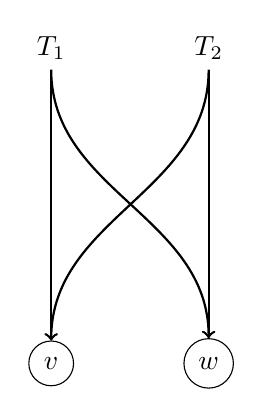
\begin{tikzpicture}
      \node (t1) at (-1,0) {$T_1$};
      \node (t2) at (1,0)  {$T_2$};
      \node (v) [draw,shape=circle] at (-1,-4) {$v$};
      \node (w) [draw,shape=circle] at (1,-4)  {$w$};

      \draw [->, thick] (t1.south) to [out=270,in=90] (v.north);
      \draw [->, thick] (t1.south) to [out=270,in=90] (w.north);
      \draw [->, thick] (t2.south) to [out=270,in=90] (v.north);
      \draw [->, thick] (t2.south) to [out=270,in=90] (w.north);
    \end{tikzpicture}
    \caption{Sequential Consistency}
  \end{subfigure}
  \begin{subfigure}{0.3\textwidth}
    \centering
    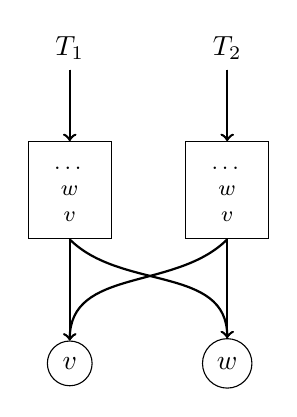
\begin{tikzpicture}
      \node (t1) at (-1,0) {$T_1$};
      \node (t2) at (1,0)  {$T_2$};
      \node (v) [draw,shape=circle] at (-1,-4) {$v$};
      \node (w) [draw,shape=circle] at (1,-4)  {$w$};

      \node (bt1) [draw] at (-1,-1.8) {\footnotesize\begin{tabular}{c} \ldots \\\midrule $w$ \\\midrule $v$ \end{tabular}};
      \node (bt2) [draw] at (1,-1.8) {\footnotesize\begin{tabular}{c} \ldots \\\midrule $w$ \\\midrule $v$ \end{tabular}};

      \draw [->, thick] (t1) to [out=270,in=90] (bt1);
      \draw [->, thick] (t1) to [out=270,in=90] (bt1);
      \draw [->, thick] (t2) to [out=270,in=90] (bt2);
      \draw [->, thick] (t2) to [out=270,in=90] (bt2);

      \draw [->, thick] (bt1.south) to [out=270,in=90] (v);
      \draw [->, thick] (bt1.south) to [out=315,in=90] (w);
      \draw [->, thick] (bt2.south) to [out=225,in=90] (v);
      \draw [->, thick] (bt2.south) to [out=270,in=90] (w);
    \end{tikzpicture}
    \caption{Total Store Order}
  \end{subfigure}
  \begin{subfigure}{0.3\textwidth}
    \centering
    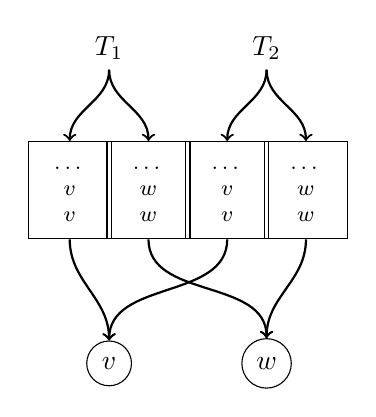
\begin{tikzpicture}
      \node (t1) at (-1,0) {$T_1$};
      \node (t2) at (1,0)  {$T_2$};
      \node (v) [draw,shape=circle] at (-1,-4) {$v$};
      \node (w) [draw,shape=circle] at (1,-4)  {$w$};

      \node (bt1v) [draw] at (-1.5,-1.8) {\footnotesize\begin{tabular}{c} \ldots \\\midrule $v$ \\\midrule $v$ \end{tabular}};
      \node (bt1w) [draw] at (-0.5,-1.8) {\footnotesize\begin{tabular}{c} \ldots \\\midrule $w$ \\\midrule $w$ \end{tabular}};
      \node (bt2v) [draw] at (0.5,-1.8) {\footnotesize\begin{tabular}{c} \ldots \\\midrule $v$ \\\midrule $v$ \end{tabular}};
      \node (bt2w) [draw] at (1.5,-1.8) {\footnotesize\begin{tabular}{c} \ldots \\\midrule $w$ \\\midrule $w$ \end{tabular}};

      \draw [->, thick] (t1) to [out=270,in=90] (bt1v);
      \draw [->, thick] (t1) to [out=270,in=90] (bt1w);
      \draw [->, thick] (t2) to [out=270,in=90] (bt2v);
      \draw [->, thick] (t2) to [out=270,in=90] (bt2w);

      \draw [->, thick] (bt1v.south) to [out=270,in=90] (v);
      \draw [->, thick] (bt1w.south) to [out=270,in=90] (w);
      \draw [->, thick] (bt2v.south) to [out=270,in=90] (v);
      \draw [->, thick] (bt2w.south) to [out=270,in=90] (w);
    \end{tikzpicture}
    \caption{Partial Store Order}
  \end{subfigure}
  \caption{Example of write buffering for two threads and two \texttt{IORef}s.}
  \label{fig:wb}
\end{figure}

We divide operations into three categories: \emph{synchronised}
operations impose a \emph{memory barrier}, committing all writes;
\emph{partially synchronised} operations commit one or more writes to
the same \verb|IORef|; and \emph{unsynchronised} operations never cause
a commit.

\paragraph{Phantom threads}
For each write buffer, we introduce a \emph{phantom thread}.  When
executed, a phantom thread commits the oldest write from its
corresponding buffer.  So when using sequentially consistency, the set
of runnable threads is exactly the set of threads created by forking
which are not blocked, but when using a relaxed memory model, this is
not the case.  This may seem like an odd approach: why create new
threads to model relaxed memory?  By using phantom threads, relaxed
memory nondeterminism becomes just another aspect of scheduling
nondeterminism.  We take this approach from \cite{zhang2015}.

\section{Operational Semantics}
\label{sec:dejafu-semantics}

Fundamental to \dejafu{} is an operational semantics for Haskell
concurrency, in the form of a step function on primitive actions.
Given the current state, which we call the context, we select a thread
to execute and either indicate a failure condition, or produce a new
context.  We also produce an execution trace for the user.  Our
semantics is similar in spirit to \cite{vollmer2017}, however we model
a much larger set of operations, and support partial store order as
well as total store order.

\newcommand{\bnfeq}{\text{::=}}
\newcommand{\bnfor}{\quad\text{|}\quad}

\begin{figure}
\centering
\[
\begin{array}{lrcl}
  \multicolumn{2}{r}{tid,~tid2} &\in&\text{Thread Identifier}\\
  \multicolumn{2}{r}{id}        &\in&\text{Heap Identifier}\\
  \multicolumn{2}{r}{a}         &\in&\text{Value}\\
  \multicolumn{2}{r}{c}         &\in&\text{Action Value}\\
  \multicolumn{2}{r}{e}         &\in&\text{Exception Value}\\
  \multicolumn{2}{r}{i,~n}      &\in&\mathbb{N}_{1}\\\\
%
  \text{Execution Context}  &\texttt{X}&\bnfeq&\langle \texttt{C},~\texttt{B},~\texttt{H},~\texttt{T} \rangle\\
  \text{Capabilities}       &\texttt{C}&\bnfeq&n\\
  \text{Buffer (TSO)}       &\texttt{B}&\bnfeq&tid \hookrightarrow [\langle id,~a \rangle]\\
  \text{Buffer (PSO)}       &\texttt{B}&\bnfeq&\langle tid,~id \rangle \hookrightarrow [a]\\
  \text{Heap}               &\texttt{H}&\bnfeq&id \hookrightarrow a\\
  \text{Thread Map}         &\texttt{T}&\bnfeq&tid \hookrightarrow \langle \texttt{K},~\texttt{E},~\texttt{M} \rangle\\\\
%
  \text{Actions}            &\texttt{K}&\bnfeq&c\\
  \text{Exception Handlers} &\texttt{E}&\bnfeq&[\lambda e \rightarrow c]\\
  \text{Exception Mask}     &\texttt{M}&\bnfeq&\text{Unmasked} \bnfor \text{Interruptible} \bnfor \text{Uninterruptible}\\
\end{array}
\]
\caption[The syntax of values and execution contexts.]{The syntax of values and execution contexts.  \Cref{lst:actionty} gives the definition of action values.}\label{fig:opsyntax}
\end{figure}

\paragraph{Syntax}
We express our semantics as transitions on execution contexts.
\Cref{fig:opsyntax} gives the syntax for these contexts.  A context
has a number of capabilities (\texttt{C}), a relaxed-memory buffer
(\texttt{B}), a heap (\texttt{H}), and a collection of threads
(\texttt{T}).  The representation of \texttt{B} depends on the memory
model: it is a finite mapping, either from thread identifiers to a
list of heap identifier and value pairs, or from thread and heap
identifier pairs to a list of values; see
\Cref{sec:dejafu-semantics-writes}.  \texttt{H} is a finite mapping
from identifiers to values.  \texttt{T} is a finite mapping from
identifiers to threads.  A thread has a next operation to perform
(\texttt{K}), a list of exception handlers (\texttt{E}), and a masking
state (\texttt{M}).

For some rules we include side-conditions or local definitions.  We
use Haskell syntax for these.

\begin{listing}
\centering
\begin{cminted}{haskell}
data Action n
  -- Basic multithreading
  = AFork String ((forall b. ConcT n b -> ConcT n b) -> Action n)
      (ThreadId -> Action n)
  | AGetNumCapabilities     (Int -> Action n)
  | ASetNumCapabilities Int        (Action n)
  | AMyTId (ThreadId -> Action n)
  | ALift  (n a)  (a -> Action n)
  | AYield             (Action n)
  | ADelay             (Action n)
  | AReturn            (Action n)
  | AStop

  -- IORefs and relaxed memory
  | forall a.   ANewIORef     String           a (ModelIORef n a -> Action n)
  | forall a.   AReadIORef    (ModelIORef n a)                (a -> Action n)
  | forall a.   AReadIORefCas (ModelIORef n a)    (ModelTicket a -> Action n)
  | forall a.   AWriteIORef   (ModelIORef n a) a                   (Action n)
  | forall a b. AModIORef     (ModelIORef n a) (a -> (a, b))  (b -> Action n)
  | forall a b. AModIORefCas  (ModelIORef n a) (a -> (a, b))  (b -> Action n)
  | forall a.   ACasIORef (ModelIORef n a) (ModelTicket a) a
      ((Bool, ModelTicket a) -> Action n)
  | ACommit ThreadId IORefId

  -- MVars
  | forall a. ANewMVar     String            (ModelMVar n a -> Action n)
  | forall a. APutMVar     (ModelMVar n a) a                  (Action n)
  | forall a. ATakeMVar    (ModelMVar n a)               (a -> Action n)
  | forall a. AReadMVar    (ModelMVar n a)               (a -> Action n)
  | forall a. ATryPutMVar  (ModelMVar n a) a          (Bool -> Action n)
  | forall a. ATryTakeMVar (ModelMVar n a)         (Maybe a -> Action n)
  | forall a. ATryReadMVar (ModelMVar n a)         (Maybe a -> Action n)

  -- Exceptions
  | forall e.   Exception e => AThrow e
  | forall e.   Exception e => AThrowTo ThreadId e (Action n)
  | forall a e. Exception e => ACatching (e -> ConcT n a) (ConcT n a)
      (a -> Action n)
  | forall a.   AMasking MaskingState
      ((forall b. ConcT n b -> ConcT n b) -> ConcT n a) (a -> Action n)
  | AResetMask   MaskingState (Action n)
  | APopCatching              (Action n)

  -- STM
  | forall a. AAtom (ModelSTM n a) (a -> Action n)
\end{cminted}
\caption{The primitive concurrency actions.}\label{lst:actionty}
\end{listing}

\paragraph{Primitive actions}
\Cref{lst:actionty} gives the primitive actions for concurrency.
Execution happens in the context of an underlying monad, the \verb|n|
parameter to the \verb|Action| type.  This monad is usually \verb|IO|,
but can be any \verb|MonadConc|.  In these semantics we only use this
monad for the \verb|ALift| action.  \dejafu{} communicates the result
of the computation back to the caller by inserting an \verb|ALift|
action which writes the result of the main thread to a mutable
reference just before termination.

Our implementation of model execution is more similar to cooperative
multitasking than pre-emptive multitasking: if evaluating a primitive
action fails to terminate, the entire computation locks up.

\paragraph{Simplifications and omissions}
The semantic rules we present are for the small-step behaviour.  They
are tied together by a scheduling loop which we do not present here.
This scheduling loop picks a thread to step, steps it, and continues
until every thread is blocked or the main thread terminates.

For presentation purposes, we omit some of the complexities of the
implementation.  We omit building the execution trace, and we omit the
definition of helper functions, but explain them when first used.
Furthermore, while we present the heap here as a heterogeneous map, in
practice we implement it using real mutable references.

\newcommand{\semfullthread}[3]{\langle\texttt{#1}, \texttt{#2}, \texttt{#3}\rangle}
\newcommand{\semthread}[1]{\semfullthread{#1}{E}{M}}

\newcommand{\semlfullrule}[4]{\langle\texttt{C}_{#1}, \texttt{B}_{#2}, \texttt{H}_{#3}, \texttt{T}_{\left[\texttt{tid} \mapsto \semthread{#4}\right]}\rangle}
\newcommand{\semlheaprule}[2]{\semlfullrule{}{}{[\texttt{id} \mapsto \texttt{#2}]}{#1}}
\newcommand{\semlrule}[1]{\semlfullrule{}{}{}{#1}}

\subsection{Basic Concurrency}

\begin{figure}
\centering
\begin{tabular}{r@{\hspace{0.5em}}l}
$\langle\texttt{C}, \texttt{B}, \texttt{H}, \texttt{T}_{\left[\texttt{tid} \mapsto \semfullthread{AFork \_ act c}{E}{m0}\right]}\rangle\rightarrow$&
$\langle\texttt{C}, \texttt{B}, \texttt{H}, \texttt{T}_{[\texttt{tid} \mapsto \semfullthread{c tid2}{E}{m0};~\texttt{tid2} \mapsto \texttt{new}]}\rangle$\\
\multicolumn{2}{l}{where \texttt{tid2} is not in the domain of \texttt{T}}\\
\multicolumn{2}{l}{\hphantom{where }$\texttt{reset m'} = \texttt{\textbackslash k -> AResetMask m' k}$}\\
\multicolumn{2}{l}{\hphantom{where }$\texttt{umask mb} = \texttt{reset Unmasked >> mb >> \textbackslash b -> reset m0 >> pure b}$}\\
\multicolumn{2}{l}{\hphantom{where }$\texttt{new} = \langle\texttt{act umask}, \texttt{[]}, \texttt{m0}\rangle$}\\
& \\
$\semlrule{AGetNumCapabilities c}\rightarrow$&
$\langle\texttt{C}, \texttt{B}, \texttt{H}, \texttt{T}_{[\texttt{tid} \mapsto \semthread{c C}]}\rangle$\\
$\semlrule{ASetNumCapabilities i c}\rightarrow$&
$\langle\texttt{i}, \texttt{B}, \texttt{H}, \texttt{T}_{[\texttt{tid} \mapsto \semthread{c}]}\rangle$\\
$\semlrule{AMyTId c}\rightarrow$&
$\langle\texttt{C}, \texttt{B}, \texttt{H}, \texttt{T}_{[\texttt{tid} \mapsto \semthread{c tid}]}\rangle$\\
$\semlrule{AYield c}\rightarrow$&
$\langle\texttt{C}, \texttt{B}, \texttt{H}, \texttt{T}_{[\texttt{tid} \mapsto \semthread{c}]}\rangle$\\
$\semlrule{ADelay c}\rightarrow$&
$\langle\texttt{C}, \texttt{B}, \texttt{H}, \texttt{T}_{[\texttt{tid} \mapsto \semthread{c}]}\rangle$\\
$\semlrule{AReturn c}\rightarrow$&
$\langle\texttt{C}, \texttt{B}, \texttt{H}, \texttt{T}_{[\texttt{tid} \mapsto \semthread{c}]}\rangle$\\
$\semlrule{ALift na c}\rightarrow$&
$\langle\texttt{C}, \texttt{B}, \texttt{H}, \texttt{T}_{[\texttt{tid} \mapsto \semthread{na >>= c}]}\rangle$\\
$\semlrule{AStop}\rightarrow$&
$\langle\texttt{C}, \texttt{B}, \texttt{H}, \texttt{T}_{[\texttt{tid} \mapsto \varnothing]}\rangle$
\end{tabular}
\caption{Transition semantics of basic multithreading actions.}\label{fig:sem_multithreading}
\end{figure}

\Cref{fig:sem_multithreading} shows the semantics for the basic
multithreading operations.  These rules do not involve memory, so they
leave the relaxed-memory buffer and heap untouched.  We write
$\texttt{M}_{[\texttt{k} \mapsto \texttt{v}]}$ to denote a new map
which maps the key \texttt{k} to the value \texttt{v}.

Rather than have one primitive action for each of the \verb|fork|-like
functions, we only provide \verb|AFork|, which implements
\verb|forkWithUnmask| for named threads, and implement the others in
terms of this.  We do not model which capability a thread is executing
on, so we do not also need an ``\verb|AForkOn|'' action.

The \verb|ALift| and \verb|AStop| actions are a little unlike the
others.  \verb|ALift| causes a Haskell-level effect to occur by
executing some action in the underlying monad.  \verb|AStop| has no
continuation, we use $\texttt{T}_{[\texttt{tid}\mapsto\varnothing]}$
to mean that the thread is deleted.

\paragraph{\texttt{IORef} operations}
\Cref{fig:sem_ioref} shows the semantics for the \verb|IORef|
operations.  We represent a \verb|IORef| as reference to a pair of a
number of commits and a latest value.  We present the rules for
writing to and committing to an \verb|IORef|, which depends on the
memory model, in \Cref{sec:dejafu-semantics-writes}

We use $\texttt{H} \oplus \texttt{B}$ to mean a new heap with all
buffered writes committed, nondeterministically, in some order
permitted by the memory model.  This is a memory barrier.  We use
$\texttt{H} \oplus \texttt{B}_{[\texttt{tid}]}$ to mean that only the
buffered writes from thread \verb|tid| are committed.  Under
sequential consistency there are no buffered writes, so
$\texttt{H} \oplus \texttt{\_} = \texttt{H}$.

\paragraph{\texttt{MVar} operations}
\Cref{fig:sem_mvar} shows the semantics for the \verb|MVar|
operations.  We represent an \verb|MVar| as a reference to a
\verb|Maybe| value.  These operations enforce a memory barrier, and
some may cause the thread to block.  An action can enforce a memory
barrier even if it blocks.  We model blocking by not changing the
continuation for the chosen thread.

\paragraph{Exceptions and masking}
\Cref{fig:sem_exc} shows the semantics for the exception and masking
operations.  The \verb|raise| function pops from a stack of exception
handlers until it finds a handler for the given exception.  The
\verb|interruptible| function checks if the given thread can be
interrupted with an exception.  A thread can be interrupted if its
masking state is ``unmasked'', or if its masking state is
``interruptible'' and it is blocked.

The \verb|AMasking| action is similar to \verb|AFork|: it runs an
action after passing an argument to change the masking state.
However, unlike \verb|AFork|, \verb|AMasking| runs the action in the
current thread rather than creating a new one.

\begin{figure}
\centering
\begin{tabular}{r@{\hspace{0.5em}}l}
$\semlrule{ANewIORef \_ a c}\rightarrow$&
$\langle\texttt{C}, \texttt{B}, \texttt{H}_{[\texttt{id} \mapsto \texttt{(0, a)}]}, \texttt{T}_{[\texttt{tid} \mapsto \semthread{c id}]}\rangle$ \\
\multicolumn{2}{l}{where \texttt{id} is not in the domain of \texttt{H}}\\
& \\
$\semlrule{AReadIORef id c}\rightarrow$&
$\langle\texttt{C}, \texttt{B}, \texttt{H}, \texttt{T}_{[\texttt{tid} \mapsto \semthread{c x}]}\rangle$ \\
\multicolumn{2}{l}{where $\texttt{(\_, x)} = (\texttt{H} \oplus \texttt{B}_{[\texttt{tid}]})_{[\texttt{id}]}$}\\
& \\
$\semlrule{AReadIORefCAS id c}\rightarrow$&
$\langle\texttt{C}, \texttt{B}, \texttt{H}, \texttt{T}_{[\texttt{tid} \mapsto \semthread{c (Ticket id n x)}]}\rangle$ \\
\multicolumn{2}{l}{where $\texttt{(n, x)} = (\texttt{H} \oplus \texttt{B}_{[\texttt{tid}]})_{[\texttt{id}]}$}\\
& \\
$\semlrule{AModIORef id f c}\rightarrow$&\\
\multicolumn{2}{r}{$\langle\texttt{C}, \varnothing, (\texttt{H} \oplus \texttt{B})_{[\texttt{id} \mapsto \texttt{(n+1, f a)}]}, \texttt{T}_{[\texttt{tid} \mapsto \semthread{c}]}\rangle$}\\
\multicolumn{2}{l}{where $\texttt{(n, a)} = \texttt{H} \oplus \texttt{B}_{[\texttt{tid}]}$}\\
& \\
$\semlrule{AModIORefCAS id f c}\rightarrow$&\\
\multicolumn{2}{r}{$\langle\texttt{C}, \varnothing, (\texttt{H} \oplus \texttt{B})_{[\texttt{id} \mapsto \texttt{(n+1, f a)}]}, \texttt{T}_{[\texttt{tid} \mapsto \semthread{c}]}\rangle$}\\
\multicolumn{2}{l}{where $\texttt{(n, a)} = (\texttt{H} \oplus \texttt{B})_{[\texttt{id}]}$}\\
& \\
\multicolumn{2}{l}{$\semlrule{ACasIORef id (Ticket id n \_) a} \rightarrow$}\\
\multicolumn{2}{r}{$\langle\texttt{C}, \varnothing, (\texttt{H} \oplus \texttt{B})_{[\texttt{id} \mapsto \texttt{(n+1, a)}]}, \texttt{T}_{[\texttt{tid} \mapsto \semthread{c (True, Ticket id (n+1) a)}]}\rangle$}\\
\multicolumn{2}{l}{if $\texttt{n} = \texttt{n0}$}\\
\multicolumn{2}{l}{where $\texttt{(n0, \_)} = (\texttt{H} \oplus \texttt{B})_{[\texttt{id}]}$}\\
& \\
\multicolumn{2}{l}{$\semlrule{ACasIORef id (Ticket id n \_) \_} \rightarrow$}\\
\multicolumn{2}{r}{$\langle\texttt{C}, \varnothing, \texttt{H} \oplus \texttt{B}, \texttt{T}_{[\texttt{tid} \mapsto \semthread{c (False, Ticket id n0 a0)}]}\rangle$}\\
\multicolumn{2}{l}{if $\texttt{n} \neq \texttt{n0}$}\\
\multicolumn{2}{l}{where $\texttt{(n0, a0)} = (\texttt{H} \oplus \texttt{B})_{[\texttt{id}]}$}\\
&
\end{tabular}
\caption{Transition semantics of \texttt{IORef} actions.}\label{fig:sem_ioref}
\end{figure}

\begin{figure}
\centering
\begin{tabular}{r@{\hspace{0.5em}}l}
\multicolumn{2}{r}{$\semlrule{ANewMVar \_ c} \rightarrow \langle\texttt{C}, \texttt{B}, \texttt{H}_{[\texttt{id} \mapsto \texttt{Nothing}]}, \texttt{T}_{[\texttt{tid} \mapsto \semthread{c id}]}\rangle$}\\
\multicolumn{2}{l}{where \texttt{id} is not in the domain of \texttt{H}}\\
& \\
$\semlheaprule{APutMVar id \_ \_}{Just \_}$\hfill$\rightarrow$&
$\langle\texttt{C}, \varnothing, \texttt{H} \oplus \texttt{B}, \texttt{T}\rangle$\\
& \\
$\semlheaprule{APutMVar id a c}{Nothing}$\hfill$\rightarrow$&\\
\multicolumn{2}{r}{$\langle\texttt{C}, \varnothing, \texttt{H}_{[\texttt{id} \mapsto \texttt{Just a}]} \oplus \texttt{B}, \texttt{T}_{[\texttt{tid} \mapsto \semthread{c}]}\rangle$}\\
& \\
$\semlheaprule{ATakeMVar id c}{Just x}$\hfill$\rightarrow$&\\
\multicolumn{2}{r}{$\langle\texttt{C}, \varnothing, \texttt{H}_{[\texttt{id} \mapsto \texttt{Nothing}]} \oplus \texttt{B}, \texttt{T}_{[\texttt{tid} \mapsto \semthread{c x}]}\rangle$}\\
& \\
$\semlheaprule{ATakeMVar id \_ \_}{Nothing}$\hfill$\rightarrow$&
$\langle\texttt{C}, \varnothing, \texttt{H} \oplus \texttt{B}, \texttt{T}\rangle$\\
& \\
$\semlheaprule{AReadMVar id c}{Just x}\rightarrow$&
$\langle\texttt{C}, \varnothing, \texttt{H} \oplus \texttt{B}, \texttt{T}_{[\texttt{tid} \mapsto \semthread{c x}]}\rangle$\\
& \\
$\semlheaprule{AReadMVar id \_ \_}{Nothing}$\hfill$\rightarrow$&
$\langle\texttt{C}, \varnothing, \texttt{H} \oplus \texttt{B}, \texttt{T}\rangle$\\
& \\
$\semlheaprule{ATryPutMVar id c}{Just \_}$\hfill$\rightarrow$&\\
\multicolumn{2}{r}{$\langle\texttt{C}, \varnothing, \texttt{H} \oplus \texttt{B}, \texttt{T}_{[\texttt{tid} \mapsto \semthread{c False}]}\rangle$}\\
& \\
$\semlheaprule{ATryPutMVar id a c}{Nothing}$\hfill$\rightarrow$&\\
\multicolumn{2}{r}{$\langle\texttt{C}, \varnothing, \texttt{H}_{[\texttt{id} \mapsto \texttt{Just a}]} \oplus \texttt{B}, \texttt{T}_{[\texttt{tid} \mapsto \semthread{c True}]}\rangle$}\\
& \\
$\semlheaprule{ATryTakeMVar id c}{Just x}$\hfill$\rightarrow$&\\
\multicolumn{2}{r}{$\langle\texttt{C}, \varnothing, \texttt{H}_{[\texttt{id} \mapsto \texttt{Nothing}]} \oplus \texttt{B}, \texttt{T}_{[\texttt{tid} \mapsto \semthread{c (Just x)}]}\rangle$}\\
& \\
$\semlheaprule{ATryTakeMVar id c}{Nothing}$\hfill$\rightarrow$&\\
\multicolumn{2}{r}{$\langle\texttt{C}, \varnothing, \texttt{H} \oplus \texttt{B}, \texttt{T}_{[\texttt{tid} \mapsto \semthread{c Nothing}]}\rangle$}\\
& \\
$\semlheaprule{ATryReadMVar id c}{x}\rightarrow$&
$\langle\texttt{C}, \varnothing, \texttt{H} \oplus \texttt{B}, \texttt{T}_{[\texttt{tid} \mapsto \semthread{c x}]}\rangle$
\end{tabular}
\caption{Transition semantics of \texttt{MVar} actions.}\label{fig:sem_mvar}
\end{figure}

\begin{figure}
\centering
\begin{tabular}{r@{\hspace{0.5em}}l}
$\langle\texttt{C}, \texttt{B}, \texttt{H}, \texttt{T}_{\left[\texttt{tid} \mapsto \semfullthread{AThrow e}{hs}{M}\right]}\rangle\rightarrow$&
$\langle\texttt{C}, \texttt{B}, \texttt{H}, \texttt{T}_{[\texttt{tid} \mapsto \varnothing]}\rangle$ \\
\multicolumn{2}{l}{if $\texttt{null (raise hs e)}$}\\
& \\
$\langle\texttt{C}, \texttt{B}, \texttt{H}, \texttt{T}_{\left[\texttt{tid} \mapsto \semfullthread{AThrow e}{hs}{M}\right]}\rangle\rightarrow$&
$\langle\texttt{C}, \texttt{B}, \texttt{H}, \texttt{T}_{[\texttt{tid} \mapsto \semfullthread{h e}{hs}{M}]}\rangle$ \\
\multicolumn{2}{l}{if \texttt{not (null (raise hs e))}}\\
\multicolumn{2}{l}{where \texttt{(h:hs)} = \texttt{raise hs e}}\\
& \\
$\semlrule{AThrowTo id e c}\rightarrow$\\
\multicolumn{2}{r}{$\langle\texttt{C}, \varnothing, \texttt{H} \oplus \texttt{B}, \texttt{T}_{[\texttt{tid} \mapsto \semthread{c};~\texttt{id} \mapsto \semfullthread{AThrow e}{E'}{M'}]}\rangle$}\\
\multicolumn{2}{l}{if \texttt{interruptible id}}\\
\multicolumn{2}{l}{where $\langle\texttt{\_}, \texttt{E'}, \texttt{M'}\rangle = \texttt{T}_{[\texttt{id}]}$}\\
& \\
$\semlrule{AThrowTo id \_ \_}\rightarrow$&
$\langle\texttt{C}, \varnothing, \texttt{H} \oplus \texttt{B}, \texttt{T}\rangle$\\
\multicolumn{2}{l}{if \texttt{not (interruptible id)}}\\
& \\
$\langle\texttt{C}, \texttt{B}, \texttt{H}, \texttt{T}_{\left[\texttt{tid} \mapsto \semfullthread{ACatching i inner c}{hs}{M}\right]}\rangle\rightarrow$&\\
\multicolumn{2}{r}{$\langle\texttt{C}, \texttt{B}, \texttt{H}, \texttt{T}_{[\texttt{tid} \mapsto \semfullthread{inner (APopCatching . c)}{h:hs}{M}]}\rangle$} \\
& \\
$\langle\texttt{C}, \texttt{B}, \texttt{H}, \texttt{T}_{\left[\texttt{tid} \mapsto \semfullthread{APopCatching c}{\_:hs}{M}\right]}\rangle\rightarrow$&
$\langle\texttt{C}, \texttt{B}, \texttt{H}, \texttt{T}_{[\texttt{tid} \mapsto \semfullthread{c}{hs}{M}]\rangle}$ \\
& \\
$\langle\texttt{C}, \texttt{B}, \texttt{H}, \texttt{T}_{\left[\texttt{tid} \mapsto \semfullthread{AMasking m act c}{E}{m0}\right]}\rangle\rightarrow$&\\
\multicolumn{2}{r}{$\langle\texttt{C}, \texttt{B}, \texttt{H}, \texttt{T}_{[\texttt{tid} \mapsto \semfullthread{act umask (AResetMask m0 . c)}{E}{m}]}\rangle$} \\
& \\
\multicolumn{2}{l}{where $\texttt{m0} = \texttt{T}_{[\texttt{tid}.\texttt{M}]}$}\\
\multicolumn{2}{l}{\hphantom{where }$\texttt{reset m'} = \texttt{\textbackslash k -> AResetMask m' (k)}$}\\
\multicolumn{2}{l}{\hphantom{where }$\texttt{umask mb} = \texttt{reset m0 >> mb >> \textbackslash b -> reset m >> pure b}$}\\
& \\
$\semlrule{AResetMask m c}\rightarrow$&
$\langle\texttt{C}, \texttt{B}, \texttt{H}, \texttt{T}_{[\texttt{tid} \mapsto \semfullthread{c}{E}{m}]}\rangle$
\end{tabular}
\caption{Transition semantics of exception actions.}\label{fig:sem_exc}
\end{figure}

\subsection{The Memory Model}
\label{sec:dejafu-semantics-writes}

To avoid giving all of our semantic rules which read from memory three
times, we have used the $\oplus$ operator, to denote synchronising any
buffered writes to the global memory in a nondeterministic fashion.
The behaviour of this operator depends on the memory model used.

\begin{itemize}
\item Under sequential consistency, there are no buffered writes, so
  $\texttt{H} \oplus \texttt{\_} = \texttt{H}$.
\item Under total store order, we give each thread a buffer, so
  \verb|B| is a map from thread identifiers to sequences of writes.
  Here $\texttt{H} \oplus \texttt{B}$ selects a thread with buffered
  writes nondeterministically, and pops and performs the oldest write
  from its buffer.  This process is repeated until there are no
  remaining buffered writes.
\item Under partial store order, there is a buffer for each (thread,
  \verb|IORef|) pair, but the process is otherwise the same as for
  TSO.
\end{itemize}

\paragraph{Writing to an \texttt{IORef}}
\Cref{fig:sem_ioref_relaxed_w} gives the semantic rules for writing to
an \verb|IORef|.  There is one rule for each memory model,
corresponding to the buffering strategy used.  Under sequential
consistency, the write goes straight to the heap; under TSO, the write
is appended to the buffer for the chosen thread; and under PSO the
write is appended to the buffer for the chosen (thread, \verb|IORef|)
pair.

\paragraph{Committing buffered writes}
\Cref{fig:sem_ioref_relaxed_c} gives the semantic rules for committing
buffered \verb|IORef| writes.  There is no rule for sequential
consistency, as there are no buffered writes in that case.  Another
way to think of the $\oplus$ operator is that it performs all possible
commit actions.

\begin{figure}
\centering
\begin{tabular}{r@{\hspace{0.5em}}l}
\multicolumn{2}{c}{$\semlrule{AWriteIORef id a c}\rightarrow\langle\texttt{C}, \texttt{B}, \texttt{H}_{[\texttt{id} \mapsto \texttt{(0, a)}]}, \texttt{T}_{[\texttt{tid} \mapsto \semthread{c}]}\rangle$}\\
\multicolumn{2}{l}{if using sequential consistency}\\
& \\
$\semlfullrule{}{[\texttt{tid} \mapsto \texttt{buf}]}{}{AWriteIORef id a c}\rightarrow$&\\
\multicolumn{2}{r}{$\langle\texttt{C}, \texttt{B}_{[\texttt{tid} \mapsto \texttt{(buf ++ (id, a))}]}, \texttt{H}, \texttt{T}_{[\texttt{tid} \mapsto \semthread{c}]}\rangle$}\\
\multicolumn{2}{l}{if using total store order}\\
& \\
$\semlfullrule{}{[\texttt{(tid, id)} \mapsto \texttt{buf}]}{}{AWriteIORef id a c}\rightarrow$&\\
\multicolumn{2}{r}{$\langle\texttt{C}, \texttt{B}_{[\texttt{(tid, id)} \mapsto \texttt{(buf ++ a)}]}, \texttt{H}, \texttt{T}_{[\texttt{tid} \mapsto \semthread{c}]}\rangle$}\\
\multicolumn{2}{l}{if using partial store order}
\end{tabular}
\caption{Transition semantics of writing to \texttt{IORef}s.}\label{fig:sem_ioref_relaxed_w}
\end{figure}

\begin{figure}
\centering
\begin{tabular}{r@{\hspace{0.5em}}l}
$\langle\texttt{C}, \texttt{B}_{[\texttt{tid} \mapsto \texttt{((id, a):buf)}]}, \texttt{H}_{[\texttt{id} \mapsto \texttt{(n, \_)}]}, \texttt{T}\rangle \rightarrow$&
$\langle\texttt{C}, \texttt{B}_{[\texttt{tid} \mapsto \texttt{buf}]}, \texttt{H}_{[\texttt{id} \mapsto \texttt{(n+1, a)}]}, \texttt{T}\rangle$ \\
\multicolumn{2}{l}{if using total store order}\\
$\langle\texttt{C}, \texttt{B}_{[\texttt{(tid, id)} \mapsto \texttt{(a:buf)}]}, \texttt{H}_{[\texttt{id} \mapsto \texttt{(n, \_)}]}, \texttt{T}\rangle \rightarrow$&
$\langle\texttt{C}, \texttt{B}_{[\texttt{(tid, id)} \mapsto \texttt{buf}]}, \texttt{H}_{[\texttt{id} \mapsto \texttt{(n+1, a)}]}, \texttt{T}\rangle$ \\
\multicolumn{2}{l}{if using partial store order}
\end{tabular}
\caption{Transition semantics of committing \texttt{IORef} writes.}\label{fig:sem_ioref_relaxed_c}
\end{figure}

\subsection{Software Transactional Memory}

Here we only give the semantics of the \verb|AAtom| action, a full
operational semantics of STM is given in \cite{harris2005}.  The STM
semantics are small-step reductions of the form
$M; \Theta, \Delta \Rightarrow N; \Theta', \Delta'$, where $M$ and $N$
are Haskell expressions, $\Theta$ is the heap, and $\Delta$ is the set
of \verb|TVar| variables which have been accessed.  We use
$\xRightarrow{*}$ to denote a sequence of multiple small-step
reductions.

\begin{figure}[h]
\centering
\begin{prooftree}
\AxiomC{$\texttt{stm};~\texttt{H} \oplus \texttt{B}, \varnothing \xRightarrow{*} \texttt{return x};~\texttt{H'}, \texttt{\_}$}
\UnaryInfC{$\semlrule{AAtom stm c} \rightarrow \langle\texttt{C}, \varnothing, \texttt{H'}, \texttt{T}_{[\texttt{tid} \mapsto \semthread{c x}]}\rangle$}
\end{prooftree}

\begin{prooftree}
\AxiomC{$\texttt{stm};~\texttt{H} \oplus \texttt{B}, \varnothing \xRightarrow{*} \texttt{throw x};~\texttt{H'}, \texttt{\_}$}
\UnaryInfC{$\semlrule{AAtom stm \_} \rightarrow \langle\texttt{C}, \varnothing, \texttt{H'}, \texttt{T}_{[\texttt{tid} \mapsto \semthread{AThrow x}]}\rangle$}
\end{prooftree}

\begin{prooftree}
\AxiomC{$\texttt{stm};~\texttt{H} \oplus \texttt{B}, \varnothing \xRightarrow{*} \texttt{retry};~\texttt{\_}, \texttt{\_}$}
\UnaryInfC{$\semlrule{AAtom stm \_} \rightarrow \langle\texttt{C}, \varnothing, \texttt{H} \oplus \texttt{B}, \texttt{T}\rangle$}
\end{prooftree}
\caption{Transition semantics for \texttt{AAtom}.}\label{fig:sem_aatom}
\end{figure}

\Cref{fig:sem_aatom} gives the semantics of executing transactions.
Executing an STM transaction enforces a memory barrier, and writes
inside the transaction are synchronised.  If the transaction reduces
to a \verb|throw| expression, the exception is re-thrown in the
thread.  As in the \verb|MVar| and exception semantics, a transaction
which blocks still imposes a memory barrier.

\FloatBarrier
\section{Testing Concurrent Programs}
\label{sec:dejafu-testing}

\dejafu{} uses a combination of DPOR and schedule bounding to test
programs by default.  Controlled random scheduling using a fixed
number of executions is also available.  The testing algorithm to use,
and its configuration, is controlled with the \verb|Settings|
value~\sref{dejafu-whatis}.

\begin{figure}
  \centering
  \footnotesize
  \begin{tabular}{R{4cm}@{\hspace{0.5em}}L{8cm}}
    \texttt{atomicModifyIORef r \_} $\dependent$& \texttt{x}
      \hfill if \texttt{x} uses \texttt{r} \\
    \texttt{atomically x} $\dependent$& \texttt{atomically y}
      \hfill if \texttt{x} writes to a \texttt{TVar} which \texttt{y} accesses \\
    \texttt{casIORef r \_} $\dependent$& \texttt{x}
      \hfill if \texttt{x} uses \texttt{r} \\
    \texttt{commit \_} $\dependent$& \texttt{b}
      \hfill if \texttt{b} enforces a memory barrier \\
    \texttt{commit r} $\dependent$& \texttt{writeIORef r}
      \hfill if \texttt{r} has no buffered writes \\
    \texttt{commit r} $\dependent$& \texttt{x}
      \hfill if \texttt{x} uses \texttt{r} and is not a \texttt{writeIORef r} \\
    \texttt{crefRead r} $\dependent$& \texttt{b}
      \hfill if \texttt{b} enforces a memory barrier and \texttt{r} has buffered writes \\
    \texttt{crefRead r} $\dependent$& \texttt{x}
      \hfill if \texttt{x} uses \texttt{r} and is not a \texttt{crefRead r} \\
    \texttt{liftIO \_} $\dependent$& \texttt{liftIO \_} \\
    \texttt{modifyIORefCAS r \_} $\dependent$& \texttt{x}
      \hfill if \texttt{x} uses \texttt{r} \\
    \texttt{mvarRead v} $\dependent$& \texttt{mvarRead v}
      \hfill if \texttt{v} is full \\
    \texttt{mvarRead v} $\dependent$& \texttt{mvarWrite v} \\
    \texttt{mvarWrite v} $\dependent$& \texttt{mvarWrite v}
      \hfill if \texttt{v} is empty \\
    \texttt{setNumCapabilities \_} $\dependent$& \texttt{getNumCapabilities} \\
    \texttt{setNumCapabilities \_} $\dependent$& \texttt{setNumCapabilities \_} \\
    \texttt{throwTo tgt} $\dependent$& \texttt{x}
      \hfill if \texttt{x} is on thread \texttt{tgt} and can be interrupted \\
    \texttt{writeIORef r \_} $\dependent$& \texttt{x}
      \hfill if \texttt{x} uses \texttt{r} and is not a \texttt{commit r} \\
    \texttt{x} $\dependent$& \texttt{y}
      \hfill if \texttt{y} $\dependent$ \texttt{x}
  \end{tabular}
  \caption[The \dejafu{} dependency relation.]{The \dejafu{} dependency relation.  A \texttt{commit} commits one buffered write to a \texttt{IORef}.  A \texttt{crefRead} is a \texttt{readIORef} or a \texttt{readForCAS}.  An \texttt{mvarWrite} is a \texttt{putMVar} or a \texttt{tryPutMVar}.  An \texttt{mvarRead} is a \texttt{takeMVar}, \texttt{tryTakeMVar}, \texttt{readMVar}, or \texttt{tryReadMVar}.}\label{fig:deprel}
\end{figure}

\paragraph{Dependency relation}
DPOR uses a dependency relation between pairs of actions.  Two actions
are dependent if the order in which they are performed matters.  This
relation may have false positives, but cannot have false negatives.
False positives lead to exploring redundant executions, false
negatives lead to missing distinct ones.

For ease of explanation, DPOR algorithms in the literature are
presented for small languages.  A paper will typically start with a
sentence like ``we assume a core concurrent language of reads and
writes to shared variables, and locks.''  For example, in
\cite{coons2013} two actions are said to be dependent if they are
actions of the same thread, or they are both actions on the same
shared variable and at least one is a write.  The Haskell concurrency
API is richer than this, and the implicit dependencies between actions
(such as which actions impose a memory barrier) are not documented.

\Cref{fig:deprel} shows the dependency relation we use in \dejafu{}.
We use a conditional dependency relation \parencite{godefroid1993}.
Whether two actions are dependent depends on an approximation of the
current state: we record which \verb|IORef|s have buffered writes,
whether each \verb|MVar| is full or empty, and what the masking state
of every thread is.  A conditional dependency relation allows more
precise decisions.

\begin{figure}
  \centering
  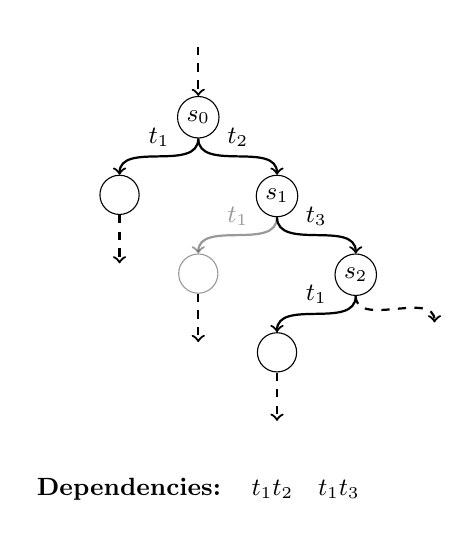
\begin{tikzpicture}[ball/.style = {circle, draw, align=center, anchor=north, inner sep=0, text width=0.5cm}]
    \node[ball]              (A) at (0,0)   {\small $s_0$};
    \node[ball]              (B) at (-1,-1) {};
    \node[ball]              (C) at (1,-1)  {\small $s_1$};
    \node[ball, opacity=0.4] (D) at (0,-2)  {};
    \node[ball]              (E) at (2,-2)  {\small $s_2$};
    \node[ball]              (F) at (1,-3)  {};

    \node (init) at (0,0.75)   {};
    \node (end1) at (-1,-2.25) {};
    \node (end2) at (0,-3.25)  {};
    \node (end3) at (3,-3)     {};
    \node (end4) at (1,-4.25)  {};
    \draw[->, thick, draw, dashed] (init.south) to [out=270,in=90] (A.north);
    \draw[->, thick, draw, dashed] (B.south) to [out=270,in=90] (end1.north);
    \draw[->, thick, draw, dashed] (D.south) to [out=270,in=90] (end2.north);
    \draw[->, thick, draw, dashed] (E.south) to [out=270,in=90] (end3.north);
    \draw[->, thick, draw, dashed] (F.south) to [out=270,in=90] (end4.north);

    \draw[->, thick, draw]              (A.south) to [out=270,in=90] node[midway,above] {\small $t_1$} (B.north);
    \draw[->, thick, draw]              (A.south) to [out=270,in=90] node[midway,above] {\small $t_2$} (C.north);
    \draw[->, thick, draw, opacity=0.4] (C.south) to [out=270,in=90] node[midway,above] {\small $t_1$} (D.north);
    \draw[->, thick, draw]              (C.south) to [out=270,in=90] node[midway,above] {\small $t_3$} (E.north);
    \draw[->, thick, draw]              (E.south) to [out=270,in=90] node[midway,above] {\small $t_1$} (F.north);

    \node (note) at (0,-5) {
      \small \textbf{Dependencies:} \hspace{0.1cm} $t_1 \independent t_2$ \hspace{0.1cm} $t_1 \dependent t_3$
    };
  \end{tikzpicture}
  \caption[The sleep set optimisation.]{The sleep set optimisation.  Transition $t_1$ may be pruned in state $s_1$ but not in state $s_2$.  The transition has been explored from state $s_0$ and there is no dependent transition between states $s_0$ and $s_1$, but there is between states $s_0$ and $s_2$.  Adapted from \cite{coons2013}.}\label{fig:sleep}
\end{figure}

\paragraph{Sleep sets}
The sleep set optimisation \parencite{godefroid1996} is a complementary
approach to DPOR which we use to further reduce schedules explored.
The intuition is as follows: if we are in a state $s_{0}$ and have a
choice of two scheduling decisions, $t_{1}$ and $t_{2}$, after trying
out $t_{1}$ there is no point in making the sequence of decisions
$t_{2}t_{1}$ from $s_{0}$, unless $t_{1} \dependent t_{2}$.  All
states reachable from $t_{1}$ have already been explored, so the only
way a new state could arise is if $t_{1}$ had a different effect,
which will only be the case if a dependent transition has been taken.
\Cref{fig:sleep} shows this graphically.

Formally, we augment each state $s$ with a \emph{sleep set},
containing transitions enabled in $s$ but which we will not make.  The
initial state has an empty sleep set.  Let $T$ be the transitions that
have been selected to be explored from $s$.  We proceed as follows:
take a transition $t_{1}$ out of $T$.  The sleep set associated with
the state reached after executing $t_{1}$ from $s$ is the sleep set
associated with $s$, minus all transitions that are dependent with
$t_{1}$.  Let $t_{2}$ be a second transition taken out of $T$.  The
sleep set associated with the state reached after executing $t_{2}$
from $s$ is the sleep set associated with $s$ augmented with $t_{1}$,
minus all transitions that are dependent with $t_{2}$.  We continue
until all transitions in $T$ have been explored, at each step adding
the previously taken transitions to the sleep set of the new state,
and removing the dependent transitions.

\paragraph{Schedule bounding}
\dejafu{} supports pre-emption bounding \parencite{musuvathi2007};
fair bounding \parencite{musuvathi2008}; and depth, or length,
bounding \parencite{russell2002}.  We use a variant of the bounded
partial-order reduction algorithm~(BPOR) \parencite{coons2013},
augmented with support for relaxed memory \parencite{zhang2015}, as
our core testing algorithm.  All three bounds are enabled by default.

\paragraph{Daemon threads}
A daemon thread is a thread which is automatically killed after the
last non-daemon thread terminates.  In Haskell, every thread other
than the main thread is a daemon thread, so as soon as the main thread
terminates the whole program terminates.  This is a problem for DPOR,
as it makes the last action of the execution dependent with everything
else in the program!

\begin{listing}
\centering
\begin{cminted}{haskell}
main = do
  v <- newEmptyMVar
  fork (myThreadId >> putMVar v "hello world")
  tryReadMVar v
\end{cminted}
\caption{A program with a race condition.}\label{lst:daemon1}
\end{listing}

\Cref{lst:daemon1} gives a small concurrent program with two possible
results: \verb|Nothing|, and \verb|Just "hello world"|.  If the
scheduler favours the main thread we only see the \verb|Nothing| case,
as there is no dependency between \verb|myThreadId| and
\verb|tryReadMVar|.  Introducing a dependency between the last action
of the execution (the \verb|tryReadMVar v| in this case) and
everything else solves this problem.

\begin{listing}
\centering
\begin{cminted}{haskell}
main = do
  v <- newEmptyMVar
  fork (myThreadId >> myThreadId >> putMVar v "hello world")
  tryReadMVar v
\end{cminted}
\caption{Another program with a race condition.}\label{lst:daemon2}
\end{listing}

However, these new dependencies also present a difficulty.  In
\Cref{lst:daemon2}, the forked thread now performs \verb|myThreadId|
twice.  If the \verb|tryReadMVar| happens after the second of these,
we get the same result as if it happens after the first.  Normally,
DPOR would recognise this and prune the redundant decision, as
\verb|myThreadId| and \verb|tryReadMVar| are independent.  However, by
introducing a dependency between the final action and everything else,
we have said that it is \emph{not} redundant!  In general, introducing
a dependency like this will lead to many redundant executions which we
would otherwise avoid.

The solution we adopt is to change the scheduler.  If the scheduler
has a choice of actions, where one or more will cause the main thread
to terminate, it records each decision as a backtracking point.  By
ensuring that every decision is tried at least once, we do not need to
introduce an additional dependency between the final action of the
main thread and everything else, and can just let DPOR do its job as
usual.

By executing every thread to completion in at least one execution, we
do see some redundant schedules.  For example, if a thread does not
communicate with any other thread, then an execution which schedules
it could in principle be modified to not schedule the thread, or
perhaps even pruned entirely.

\section{Execution traces}
\label{sec:dejafu-traces}

Execution traces are not the easiest of things to read, especially if
there are many context switches.  Traces generated by random
scheduling are particularly difficult to read, which is unfortunate,
as random testing with a fixed number of executions can be effective
for finding bugs and is much faster than DPOR.

\dejafu{} contains a trace simplifier, which attempts to rewrite
traces into a shorter form.  Unlike the shrinking done in tools like
QuickCheck \parencite{claessen2000}, \dejafu{}'s trace simplification is
\emph{semantics-preserving}.  An execution trace can be rewritten into
a simpler form which is guaranteed to produce the same result, and
there is no need to run the program again to verify this.  We achieve
this by only re-ordering independent actions, using the dependency
relation.

\begin{listing}
\begin{sublisting}{\textwidth}
\centering
\begin{cminted}{text}
S0-----P1--P0-P1-S0-P2--C-S0---P2-P3-P2--S3-P0-P3-P0---S3-P0-P3-S0-
S0----P1-P0-----P2--P0--P2-P0-S2--S3-P1-P0---S1-S3----S0--
S0--------P2-P0--P3-P2-P0-P3-P2-C-S0-S3---S2--S1-C-S1-P0----
\end{cminted}
\caption{Original}\label{lst:trace_simplification_orig}
\end{sublisting}

% [layout hack]: no gap between the listings otherwise
\vspace{1.5em}

\begin{sublisting}{\textwidth}
\centering
\begin{cminted}{text}
S0----------P1---S2-----S0----S3-----S0--
S0----------P1-P2-----S0--S1--S0---S3-----S0--
S0----------P2--P3-----S0--S2---S1--P0----
\end{cminted}
\caption{Simplified}\label{lst:trace_simplification_simplified}
\end{sublisting}
\caption[The effect of trace simplification.]{Three execution traces produced by random scheduling and their simplified counterparts.}\label{lst:trace_simplification}
\end{listing}

\Cref{lst:trace_simplification} shows three execution traces generated
by random scheduling, from one of the tests in the \dejafu{}
testsuite.  These traces are displayed in a pretty-printed form which
gives just the essence of the scheduling decisions:

\begin{itemize}
\item \verb|Sn|: indicates that thread \verb|n| started executing
  after the previously executing thread blocked or terminated.
\item \verb|Pn|: indicates that thread \verb|n| started executing by
  pre-empting the previously executing thread.
\item \verb|pn|: indicates that thread \verb|n| started executing
  after the previously executing thread yielded or delayed.
\item \verb|C|: indicates the execution of a relaxed memory commit.
\item \verb|-|: indicates the execution of one primitive action.
\end{itemize}

The three original traces involve many context
switches and relaxed memory commit actions.  They are long and hard to
follow.  In contrast, the three simplified traces are much shorter,
involve far fewer context switches, and have no relaxed memory commit
actions at all.  The simplified traces are much more useful for
program comprehension.

Our trace simplification algorithm has four steps:

\begin{enumerate}
\item Rewrite the trace into lexicographic normal form.
\item Prune redundant relaxed memory commit actions.
\item Reduce context switching by pulling actions backwards.
\item Reduce context switching by pushing actions forwards.
\end{enumerate}

We repeat steps (3) and (4) until a fixed point is reached, or a fixed
number of iterations has elapsed.

\paragraph{Rewrite the trace into lexicographic normal form}
The problem of sorting sequences where only some items can be permuted
is studied in \cite{anisimov1979}.  For the case of execution traces,
this corresponds to sorting by thread identifier, only re-ordering
independent actions.  We implement this in much the same way as bubble
sort.

Recall that a Haskell program terminates when the main thread does.
So by moving actions of the main thread, thread 0, towards the
beginning we can then delete a suffix of the trace.  This is the main
way in which we can produce shorter traces.

\paragraph{Prune redundant relaxed memory commit actions}
If a commit action is followed by a memory barrier, possibly with some
independent actions in between, the commit can be removed if there are
no other buffered writes for that \verb|IORef|.  The barrier will
commit the single write anyway.

\paragraph{Reduce context switching by pulling actions backwards}
We now walk through the trace from beginning to end, looking for
opportunities to pull actions backwards.  If we have the trace
\verb|[(t1, X), (t2, Y), (t1, Z)]|, where \verb|Y| and \verb|Z| are
independent, this transformation re-orders the trace to
\verb|[(t1, X), (t1, Z), (t2, Y)]|.  We allow any number of
independent actions before the action being pulled backwards.

\paragraph{Reduce context switching by pushing actions forwards}
This is much like the ``pull back'' transformation.  We walk the
trace, looking for cases where actions can be pushed forward.  If we
have the trace \verb|[(t1, X), (t2, Y), (t1, Z)]|, where \verb|X| and
\verb|Y| are independent, this transformation re-orders the trace to
\verb|[(t2, Y), (t1, X), (t1, Z)]|.

Having both the ``pull back'' and ``push forward'' transformations is
not redundant.  If we have three actions---\verb|X|, \verb|Y|, and
\verb|Z|---it may be that \verb|X| is independent with \verb|Y| but
\verb|Z| is not, or vice versa.

\section{Soundness and Completeness}
\label{sec:dejafu-correctness}

Correctness for \dejafu{} is about two questions:

\begin{itemize}
\item Is the set of results which are possible under normal execution
  the same as the set of results which are possible under \dejafu{}?
\item Will \dejafu{} discover all of these possible results?
\end{itemize}

These two questions highlight a natural separation in the theory: the
correspondence of \dejafu{}'s concurrency semantics to those of GHC,
and the correctness of the machinery to discover new executions.

We do not attempt to formally verify the \dejafu{} implementation, but
we do have an extensive test suite.  Testing a testing tool is a
little different to testing a regular program.  Most of our tests
consist of nondeterministic programs, where we want to verify that
\dejafu{} finds precisely the behaviours we expect.

\paragraph{Property tests}
\dejafu{} is not one monolithic implementation.  It has components
which can be specified and tested in isolation.  For example, the
dependency relation must be commutative.  We use
Hedgehog \parencite{hedgehog}, a randomised property-testing library, to
check these properties of the implementation.

\paragraph{Integration tests}
Most of the tests are integration tests, consisting of a small
concurrent program and a property to check.  A failure in such an
integration test could in principle be anywhere in \dejafu{}, and so
be hard to isolate and fix, but in practice failures in different
components tend to manifest differently.  For example, a failure in
the DPOR implementation tends to manifest as invalid schedules being
generated; whereas a failure in the concurrency implementation tends
to manifest as incorrect results of individual executions.

Our integration tests fall into the following classes:

\begin{itemize}
\item Single threaded tests for the \verb|MonadConc| primitives,
  ensuring that only the single correct behaviour is observed.
\item Multi-threaded tests for the \verb|MonadConc| primitives,
  ensuring that the expected nondeterminism is observed.
\item So-called \emph{litmus tests} for the relaxed memory
  implementation, ensuring that all expected relaxed behaviours are
  observed.
\item A copy of the async library's \parencite{async} test suite, for our
  \verb|MonadConc| version.
\item A collection of refinement tests from CoCo, which we shall
  discuss in \Cref{chp:coco}.
\item Finally, a collection of regression tests for previous bugs.
\end{itemize}

\paragraph{Example programs}
Finally, we have a collection of larger integration tests which serve
also as example usages of \dejafu{}, three of which we discuss in
\Cref{sec:dejafu-casestudies}: the monad-par library
\parencite{monad_par,marlow2011}, the auto-update library
\parencite{auto_update}, and the async library \parencite{async}.

\subsection{Correct Execution}

Correctness of execution asks: can the result of an arbitrary
execution of \dejafu{}'s testing implementation can be obtained in
reality?  Furthermore, do all real-world executions correspond to a
possible execution under \dejafu{}?

\paragraph{Program behaviour}
There is no standard for concurrent Haskell.  There is only what GHC
provides.  The behaviour of many operations is clear, but for some it
is not.  \verb|IORef| operations are particularly complicated, as their
behaviour depends on the underlying memory model, which is
unspecified.  We chose TSO, and assume that the GHC optimiser or code
generator does not affect the memory model.

There are some intentional semantic differences for practical reasons.
For example, GHC can sometimes detect deadlocks involving only a
subset of the threads, and throw an exception to the threads
signalling this.  We cannot do this.

Although the behaviour of \dejafu{} is not correct with respect to
GHC-compiled behaviour in all cases, we claim it is close enough to be
useful.

\paragraph{Possible executions}
Our stepwise execution of concurrent programs allows a scheduling
decision to be made between each primitive action, which does not
correspond to how GHC handles scheduling:

\begin{displayquote}
  GHC implements pre-emptive multitasking: the execution of threads
  are interleaved in a random fashion.  More specifically, a thread may
  be pre-empted whenever it allocates some memory, which unfortunately
  means that tight loops which do no allocation tend to lock out other
  threads (this only seems to happen with pathological benchmark-style
  code, however). \parencite{control_concurrent}
\end{displayquote}

So there are executions involving the pre-emption of the evaluation of
non-terminating expressions which are possible under GHC but not under
\dejafu{}.  However, \dejafu{} is even worse than this with bottom
values.  The program in \Cref{lst:bottom} will fail to terminate, even
if the thread with the infinite computation is never scheduled, as
\dejafu{} will hang trying to compute the continuation so it can call
the scheduler.

\begin{listing}
\centering
\begin{cminted}{haskell}
bottom = do
  fork (last [1..])
  pure ()
\end{cminted}
\caption{A program that does not halt under \dejafu{} but does under GHC.}\label{lst:bottom}
\end{listing}

\subsection{Correct Testing}

Correctness of testing asks: are the schedule prefixes generated by
the DPOR machinery valid?  Furthermore, are there any possible results
for which no schedule will be generated?  This is different to the
testing framework generating every schedule, as that is precisely what
DPOR tries to avoid.

\paragraph{Prefix validity}
Executions are stored internally as a stack, shown in \Cref{lst:dpor}.
The sequence of thread IDs corresponding to this stack represents a
complete execution of the program.  There is a unique initial state,
where only the initial thread is runnable and nothing has been done.

\begin{listing}
\centering
\begin{cminted}{haskell}
data DPOR = DPOR
  { dporRunnable :: Set ThreadId
  -- ^ What threads are runnable at this step.
  , dporTodo     :: Map ThreadId Bool
  -- ^ Follow-on decisions still to make, and whether that decision
  -- was added conservatively due to the bound.
  , dporNext     :: Maybe (ThreadId, DPOR)
  -- ^ The next decision made.
  , dporDone     :: Set ThreadId
  -- ^ All transitions which have been taken from this point,
  -- including conservatively-added ones.
  , dporSleep    :: Map ThreadId ThreadAction
  -- ^ Transitions to ignore until a dependent transition happens.
  , dporTaken    :: Map ThreadId ThreadAction
  -- ^ Transitions which have been taken, excluding
  -- conservatively-added ones.
  } deriving (Eq, Show)
\end{cminted}
\caption{The DPOR state is a stack of scheduling decisions.}\label{lst:dpor}
\end{listing}

There are some well-formedness properties associated with a
\verb|DPOR| value:

\begin{enumerate}
\item Every thread in the to-do set is runnable.
\item Every thread in the done set is runnable.
\item The taken set is a subset of the done set.
\item The done and to-do sets are disjoint.
\item The next-taken thread, if there is one, is in the done set.
\end{enumerate}

These properties should hold inductively over the whole state.  We
check these invariants everywhere a \verb|DPOR| value is constructed,
and abort if the state is invalid.  In the \dejafu{} testsuite, the
execution time overhead of this checking is 3\%.

The prefixes we generate are sequences of taken decisions followed by
a single to-do decision.  By maximising the length of prefixes, we
obtain a depth-first search of the space of schedules.  Provided the
well-formedness properties hold, and the runnable sets are correctly
recorded during execution, then a generated schedule prefix will be
valid.

\paragraph{Schedule completeness}
The DPOR machinery should eventually find every possible result of a
given program.  However, as schedule bounding is involved, some
results may not be reached.  So instead we require that, for all sets
of bounds, all results possible subject to those bounds show up under
testing with the same bounds.  Our core testing algorithm satisfies
this property \parencite{coons2013}.

\section{Case Studies}
\label{sec:dejafu-casestudies}

We now discuss the process and results of applying \dejafu{} to three
Haskell libraries:

\begin{enumerate}
\item We identify and fix a deadlock in the monad-par
  library \parencite{monad_par,marlow2011}.
\item We reproduce a known deadlock in the auto-update
  library \parencite{auto_update}.
\item We use property-based testing to reproduce a known bug in the
  async library \parencite{async}.
\end{enumerate}

We chose these libraries because each is by proficient Haskell
programmers well versed with concurrency, and yet they all contain
unintentional bugs.  This shows that even those familiar with the
standard pitfalls of concurrent programming encounter problems.

None of these libraries is written using the \verb|MonadConc|
abstraction, so we had to modify the existing code before we could
test them with \dejafu{}.
\subsection{monad-par}
\label{sec:dejafu-casestudies-par}

The monad-par library \parencite{monad_par,marlow2011} provides a
traditional-looking concurrency abstraction, giving the programmer
threads and mutable state, however it is deterministic.  Determinism
is enforced by restricting shared state: it is an error to write more
than once to the same mutable variable, and read operations block
until a value has been written.  Programs written using the library
will either give a deterministic result, or terminate with a
multiple-write error.  These shared variables, called \verb|IVar|s,
implement futures \parencite{marlow2011}.  Despite its limitations, the
library can be effective in speeding up pure code \parencite{marlow2011}.

The library provides six different schedulers.  We ported the
``direct'' scheduler, a work-stealing scheduler, to the
\verb|MonadConc| typeclass.  This was a straightforward and
compiler-driven refactoring.  Changing function types to use
\verb|MonadConc| rather than \verb|IO| led to compiler errors showing
where the next changes needed to be made.  We iterated this process of
fixing errors and recompiling until the library successfully compiled
once more.  Changes were needed in two of the source files.

Some simplifications were made in the conversion process:

\begin{itemize}
\item The scheduler creates a pseudorandom number generator for each
  worker thread.  As systematic testing requires that the scheduler be
  the only source of nondeterminism, we fixed the random seeds: the
  first worker thread gets the seed zero, the second gets the seed
  one, and so on.
\item The scheduler uses the C pre-processor to choose between
  different implementations of some of its functionality.  There are
  nine flags, each of which are independent.  We only ported and
  tested the default configuration.
\item The scheduler includes some debugging code for detecting and
  reporting errors.  We removed it.
\end{itemize}

\begin{table}
  \centering
  \begin{tabular}{lrr} \toprule
    & Direct.hs & DirectInternal.hs \\ \midrule
    Language extensions & 1 & 0 \\
    Module imports & 6 & 1 \\
    Type definitions & 7 & 13 \\
    Type signatures & 32 & 7 \\
    Function renames & 2 & 0 \\
    Logic changes & 16 & 0 \\ \midrule
    \emph{Total} & 75 & 26 \\ \bottomrule
  \end{tabular}
  \caption{Breakdown of changes to port the monad-par ``direct'' scheduler.}\label{tbl:parmonad_diff}
\end{table}

\Cref{lst:parmonad} shows the original and converted versions of the
scheduler initialisation code.  As can be seen, they are similar, even
though this is a core component of a rather sophisticated library,
where the types have been changed.  \Cref{tbl:parmonad_diff} breaks
down the changes across both files.  Code changes are broken down into
``renames,'' where the concurrency library simply provides a different
name for a function, and ``logic,'' where that was not the case.  The
logic changes were either: (1) places where a call to \verb|liftIO| or
\verb|lift| was now necessary; or (2) inserting uses of
\verb|getNumCapabilities|.

\begin{listing}
\centering
\begin{cminted}{haskell}
parfilter :: (MonadConc m, NFData a) => (a -> Bool) -> [a] -> Par m [a]
parfilter _ []  = pure []
parfilter f [x] = pure (if f x then [x] else [])
parfilter f xs  = do
    let (as, bs) = halve xs
    v1 <- Par.spawn (parfilter f as)
    v2 <- Par.spawn (parfilter f bs)
    left  <- Par.get v1
    right <- Par.get v2
    pure (left ++ right)
  where
    halve xs = splitAt (length xs `div` 2) xs
\end{cminted}
\caption{An example usage of the monad-par library.}\label{lst:parmonad_example1}
\end{listing}

\Cref{lst:parmonad_example1} shows an example usage of the library.
This \verb|parfilter| function filters a list in parallel, using a
divide-and-conquer approach.  If the list is not empty or a singleton,
it is split in half and a new thread created to filter each half.  The
results of each new thread are combined to produce the overall result.
The library requires all shared state have an instance of the
\verb|NFData| typeclass, which provides an operation to evaluate data
to normal form.  The library gains its speed by evaluating data in
separate threads.

\begin{listing}
\centering
\begin{cminted}{haskell}
test_parmonad :: (MonadConc m, MonadIO m) => [Int] -> m Bool
test_parmonad xs = do
    let p x = x `mod` 2 == 0
    s <- runPar (parfilter p xs)
    pure (s == filter p xs)
\end{cminted}
\caption{A test case comparing a parallel filter to a normal filter.}\label{lst:parmonad_example2}
\end{listing}

\paragraph{Finding a deadlock}
\Cref{lst:parmonad_example2} shows a test case for \verb|parfilter|.
A parallel filter should produce the same result as a normal filter.
\Cref{tbl:parmonad_perf} shows performance measurements for our test
case, with the input list \verb|[0..5]|, in six different
configurations.  The numbers do not look so good for DPOR.  Swarm
managed to find two deadlocking executions out of 100, whereas bounded
DPOR found none in 6140.  Unbounded DPOR did not complete at all: it
rapidly consumed all the memory of the host system when keeping traces
in memory, and was still running after two days while discarding
traces.

\begin{table}
  \centering
  \begin{subtable}{\textwidth}
    \centering
    \begin{tabular}{lSSSS} \toprule
      & {Schedules} & {Deadlocks} & {Time (s)} & {Max Residency (MB)} \\ \midrule
      Bounded DPOR   & 6140 & 0 & 35.1 &            339 \\
      Unbounded DPOR &      &   &      & {$\geq$ 16GiB} \\
      Swarm          &  100 & 2 & 0.17 &             21 \\ \bottomrule
    \end{tabular}
    \caption{Keeping all execution traces in memory.}\label{tbl:parmonad_perf1}
  \end{subtable}

  % [layout hack]: no gap between the tables otherwise
  \vspace{1.5em}

  \begin{subtable}{\textwidth}
    \centering
    \begin{tabular}{lSSSS} \toprule
      & {Schedules} & {Deadlocks} & {Time (s)} & {Max Residency (kB)} \\ \midrule
      Bounded DPOR   & 6140 & 0 &           27.9 &  842 \\
      Unbounded DPOR &      &   & {$\geq$ 48hrs} &      \\
      Swarm          &  100 & 2 &           0.14 & 1600 \\ \bottomrule
    \end{tabular}
    \caption{Only keeping buggy execution traces in memory.}\label{tbl:parmonad_perf2}
  \end{subtable}
  \caption[Performance of the monad-par case study with multiple strategies.]{Performance of the monad-par case study with three different exploration tactics.  Unbounded DPOR was aborted in both cases, after consuming too many resources.}\label{tbl:parmonad_perf}
\end{table}

When we inspect one of the execution traces leading to deadlock, we
gain two clues for why DPOR performs poorly: (1) the trace is 793
entries long, but the length bound for DPOR is 250; and (2) there are
473 calls to \verb|liftIO|, \dejafu{} considers all \verb|IO| actions
dependent and so tries every possible interleaving of these.

\begin{listing}
\centering
\begin{cminted}{text}
(Continue,[],LiftIO)
(Continue,[],LiftIO)
(Continue,[],LiftIO)
(Continue,[],ReadIORef 2)
(Continue,[],LiftIO)
(Continue,[],NewMVar 7)
(Continue,[],ModIORef 4)
(Continue,[],GetNumCapabilities 2)
(Continue,[],BlockedTakeMVar 7)
\end{cminted}
\caption{The final ten entries of the deadlocking monad-par trace.}\label{lst:parmonad_example3}
\end{listing}

Following the code by eye as we read a 793-entry trace is not
realistic.  So instead, let's look at the last few entries in the
trace, shown in \Cref{lst:parmonad_example3}.  Each trace entry is a
tuple consisting of the scheduling decision made, the alternative
decisions possible, and what the thread did.  As this is right before
deadlock, it is not surprising that there are no other threads which
could be scheduled.  There are only four calls to
\verb|getNumCapabilities| in the code we ported.  We can look at each,
to find the code which matches the trace.

\begin{listing}
\centering
\begin{cminted}{haskell}
go 0 _ | _IDLING_ON =
  do m <- newEmptyMVar
     r <- modifyHotVar idle (\is -> (m:is, is))
     numCapabilities <- getNumCapabilities
     if length r == numCapabilities - 1
       then do
         mapM_ (\vr -> putMVar vr True) r
       else do
         done <- takeMVar m
         if done
           then do
             return ()
           else do
             i <- getnext (-1::Int)
             go (maxtries numCapabilities) i
\end{cminted}
\caption[The source of the deadlock in the monad-par library.]{The source of the deadlock in the monad-par library.  In the ``then'' branch of the conditional, the \texttt{idle} list is not emptied when waking every blocked thread.}\label{lst:parmonad_example4}
\end{listing}

\Cref{lst:parmonad_example4} is our match.  When a thread is unable to
steal work, it creates an empty \verb|MVar| which it adds to a shared
list, called \verb|idle|; if that list already has an entry for every
other thread, they are woken by writing a value to their \verb|MVar|;
otherwise, the thread blocks by calling \verb|takeMVar| on its new,
empty, \verb|MVar|.  The final fragment of our execution trace
corresponds to this code where \verb|length r == numCapabilities - 1|
is false.  But how can that be false?  \emph{The list is never
  emptied!}  Think about what happens if every thread reaches this
logic \emph{twice}:

\begin{enumerate}
\item \verb|n - 1| threads add themselves to the list, and block.
\item The final thread adds itself to the list, and wakes up the other
  threads.
\item \textbf{The list is not emptied, even though every thread is woken.}
\item \verb|n - 1| threads add themselves to the list, again, and
  block.
\item The final thread adds itself to the list.  It does \emph{not}
  trigger the wake-up logic, because the list is not the right length,
  and so it also blocks.
\item \textbf{Every thread is now blocked.}
\end{enumerate}

We can confirm our suspicion by checking the trace.  Each thread does
exhibit that pattern twice, so our deduction is correct.  This problem
is solved by writing \verb|[]| to \verb|idle| before waking the
threads.  The write must happen before, otherwise there is a new race
condition: one of the woken threads could add itself to the list
again, and then its \verb|MVar| be lost when the list is cleared.

\paragraph{Handling an exception}
When running our test case in a loop using \verb|IO|, to verify that
we really had fixed the problem, another issue arose which \dejafu{}
did \emph{not} find.  After a while, the main thread would be killed
by a \verb|BlockedIndefinitelyOnMVar| exception.  Such exceptions are
out of scope~\sref{dejafu-whatis-scope}, so \dejafu{} could never find
this new problem.  There is always a gap between the real system and
the model.  \dejafu{} is just one component of the Haskell
programmer's toolbox, it is not the be-all and end-all for concurrency
testing.  However, for the class of bugs which \dejafu{} can find, it
is much more effective than simply running the program in \verb|IO|
many times.

By turning on the library's debugging output, and adding some more of
our own, we were able to track the problem down to the same logic as
before, \Cref{lst:parmonad_example4}.  A thread was still getting
blocked here, despite our fix for the deadlock.  How can a thread get
blocked indefinitely there if we make sure the last thread wakes up
the others?  \emph{The number of workers is assumed to be equal to the
  number of capabilities!}  If even a single worker terminates, all
the others will block.

Fortunately, the relevant source code is not extensive.  We were able
to quickly ascertain that the library divides its workers into two
categories: there is a single main worker, which communicates the
result of the computation back to its caller and terminates when done;
and there are all the other workers.  The other workers do check if
the computation is complete, but only in certain places.  So this was
happening:

\begin{enumerate}
\item A non-main worker checks if the computation is complete, and
  sees that it is not.
\item The same worker blocks itself as usual.
\item The computation finishes, and the main worker terminates.
\item \textbf{The GHC runtime delivers an exception to the blocked
    worker.}
\end{enumerate}

It is harmless for the worker to be blocked at this point, as the
overall computation is long-complete, and the result communicated back
to the user.  However, each worker thread is given an exception
handler which throws any received exception to its creator.  In this
case, the creator was the main thread, so the whole program is
terminated.  The solution is to check if the computation has
terminated before blocking.

\begin{listing}
  \begin{sublisting}{\textwidth}
    \centering
    \begin{cminted}{haskell}
makeScheds :: Int -> IO [Sched]
makeScheds main = do
   workpools <- replicateM numCapabilities $ R.newQ
   rngs <- replicateM numCapabilities $ Random.create >>= newHotVar
   idle <- newHotVar []
   sessionFinished <- newHotVar False
   sessionStacks   <- mapM newHotVar
     (replicate numCapabilities [Session baseSessionID sessionFinished])
   activeSessions  <- newHotVar S.empty
   sessionCounter  <- newHotVar (baseSessionID + 1)
   let allscheds = [ Sched { no=x, idle, isMain=(x==main), workpool=wp,
                             scheds=allscheds, rng=rng, sessions=stck
                             sessionCounter, activeSessions
                           }
                   | x   <- [0 .. numCapabilities-1]
                   | wp  <- workpools
                   | rng <- rngs
                   | stck <- sessionStacks
                   ]
   pure allscheds
    \end{cminted}
    \caption{Original}\label{lst:parmonad_orig}
  \end{sublisting}

  % [layout hack]: no gap between the listings otherwise
  \vspace{1.5em}

  \begin{sublisting}{\textwidth}
    \centering
    \begin{cminted}{haskell}
makeScheds :: (MonadConc m, MonadIO m) => Int -> m [Sched m]
makeScheds main = do
   numCapabilities <- getNumCapabilities
   workpools <- replicateM numCapabilities $ liftIO R.newQ
   let rng i = liftIO (Random.initialize (V.singleton $ fromIntegral i))
   rngs <- mapM (\i -> rng i >>= newHotVar) [0..numCapabilities]
   idle <- newHotVar []
   sessionFinished <- newHotVar False
   sessionStacks   <- mapM newHotVar
     (replicate numCapabilities [Session baseSessionID sessionFinished])
   activeSessions  <- newHotVar S.empty
   sessionCounter  <- newHotVar (baseSessionID + 1)
   let allscheds = [ Sched { no=x, idle, isMain=(x==main), workpool=wp,
                             scheds=allscheds, rng=rng, sessions=stck
                             sessionCounter, activeSessions
                           }
                   | x   <- [0 .. numCapabilities-1]
                   | wp  <- workpools
                   | rng <- rngs
                   | stck <- sessionStacks
                   ]
   pure allscheds
    \end{cminted}
    \caption{\dejafu{}}\label{lst:parmonad_dejafu}
  \end{sublisting}
  \caption{The monad-par ``direct'' scheduler initialisation.}\label{lst:parmonad}
\end{listing}

\subsection{auto-update}

The auto-update library \parencite{auto_update} runs tasks periodically, but
only if needed.  For example, a web server may handle each request in
a new thread, and log the time that the request arrives.  Rather than
have every such new thread check the time, one thread could be created
to update a single shared \verb|IORef| every second.  However, if the
request frequency is less than once per second, this is wasted work.
The library allows defining a periodic action which only runs when
needed.

The implementation, excluding comments and imports, is reproduced in
\Cref{lst:autoupdate}.  The library defines a function,
\verb|mkAutoUpdate|, which forks a worker thread to perform the action
when required.  The function returns an \verb|IO| action to read the
current result, if necessary blocking until there is one.  The
transformation to the \verb|MonadConc| typeclass is straightforward,
and we omit it here.

\begin{listing}
\centering
\begin{cminted}{haskell}
test_autoupdate :: MonadConc m => m ()
test_autoupdate = do
  auto <- mkAutoUpdate defaultUpdateSettings
  auto
\end{cminted}
\caption{An example usage of the auto-update library.}\label{lst:autoupdate_example1}
\end{listing}

\Cref{lst:autoupdate_example1} shows an example usage of the
\verb|MonadConc| version of the library.  The
\verb|defaultUpdateSettings| value describes an auto-updater which
runs every second, producing the value \verb|()|.  An \verb|MVar| is
used to communicate to the thread that the updater should run.  Inside
the worker, a delay is used to ensure that the action is not computed
too frequently: this is what gives the rate limiting.  So we create an
auto-updater which produces \verb|()|, and immediately demand the
value.

\begin{listing}
\centering
\begin{cminted}{text}
> autocheck test_autoupdate

[fail] Never Deadlocks
        [deadlock] S0--------S1-----------S0-
[pass] No Exceptions
[fail] Consistent Result
        () S0--------S1--------p0--

        [deadlock] S0--------S1-----------S0-
\end{cminted}
\caption[Using \dejafu{} to run a collection of standard tests.]{Using \dejafu{} to run a collection of standard tests.  The \texttt{autocheck} function looks for deadlocks, uncaught exceptions in the main thread, and nondeterminism.  Each result is displayed with a simplified view of a representative execution trace.}\label{lst:autoupdate_example2}
\end{listing}

\paragraph{Testing with \dejafu{}}
\Cref{lst:autoupdate_example2} shows one way in which we can use
\dejafu{} to explore the behaviour of our small example.  The
\verb|autocheck| function looks for some common concurrency errors.
In this example, \dejafu{} discovers a deadlock.  Each result is
displayed with a simplified view of a representative execution trace.
More detailed execution traces are also available, which contain a
summary of the primitive actions which occurred and the alternative
scheduling decisions available.

We can see from the trace of the deadlock result that thread 0
executed for a while, then thread 1, then thread 0 again.  As these
are all \verb|S| points, each thread executed until it blocked.  So we
can look at the source code in \Cref{lst:autoupdate_example1} and
\Cref{lst:autoupdate} to see what Following the execution by eye, we
see this sequence of concurrency events:

\begin{enumerate}
\item Thread 0:
  \begin{enumerate}
  \item Line 16: \verb|currRef <- newIORef Nothing|
  \item Line 17: \verb|needsRunning <- newEmptyMVar|
  \item Line 18: \verb|lastValue <- newEmptyMVar|
  \item Line 20: \verb|void $ forkIO $ ...|
  \item Line 35: \verb|mval <- readIORef currRef|
  \item Line 39: \verb|void $ tryPutMVar needsRunning ()|
  \item Line 40: \verb|readMVar lastValue|
  \item \textbf{Thread 0 is now blocked, as \texttt{lastValue} is empty.}
  \end{enumerate}
\item Thread 1:
  \begin{enumerate}
  \item Line 21: \verb|takeMVar needsRunning|
  \item Line 25: \verb|writeIORef currRef $ Just a|
  \item Line 26: \verb|void $ tryTakeMVar lastValue|
  \item Line 27: \verb|putMVar lastValue a|
  \item \textbf{Thread 0 is now unblocked, as \texttt{lastValue} is full.}
  \item Line 29: \verb|threadDelay $ updateFreq us|
  \item Line 31: \verb|writeIORef currRef Nothing|
  \item Line 32: \verb|void $ takeMVar lastValue|
  \item \textbf{Thread 0 is still unblocked, even though \texttt{lastValue} is now empty again.}
  \item \textbf{Thread 1 now loops.}
  \item Line 21: \verb|takeMVar needsRunning|
  \item \textbf{Thread 1 is now blocked, as \texttt{needsRunning} is empty.}
  \end{enumerate}
\item Thread 0:
  \begin{enumerate}
  \item Line 40: \verb|readMVar lastValue|
  \item \textbf{Thread 0 is now blocked, as \texttt{lastValue} is empty.}
  \end{enumerate}
\end{enumerate}

Both threads are blocked, so the computation is deadlocked.  The other
result shown in \Cref{lst:autoupdate_example2} occurs if thread 0
starts executing after thread 1 delays.  So the root cause of this
deadlock is clear: deadlock may occur if the call to
\verb|threadDelay| on line 29 completes before the other thread
resumes execution.  Despite this bug being rather simple, not
requiring any pre-emptions at all to trigger, it arose in practice.
How easy it is to make mistakes when implementing concurrent programs!

\begin{table}
  \centering
  \begin{subtable}{\textwidth}
    \centering
    \begin{tabular}{lSSSS} \toprule
      & {Schedules} & {Deadlocks} & {Time (s)} & {Max Residency (kB)} \\ \midrule
      Bounded DPOR   &  49 & 18 & 0.006 &  119 \\
      Unbounded DPOR &  80 & 20 & 0.008 &  124 \\
      Swarm          & 100 & 20 & 0.008 & 1297 \\ \bottomrule
    \end{tabular}
    \caption{Keeping all execution traces in memory.}\label{tbl:autoupdate_perf1}
  \end{subtable}

  % [layout hack]: no gap between the tables otherwise
  \vspace{1.5em}

  \begin{subtable}{\textwidth}
    \centering
    \begin{tabular}{lSSSS} \toprule
      & {Schedules} & {Deadlocks} & {Time (s)} & {Max Residency (kB)} \\ \midrule
      Bounded DPOR   &  49 & 18 & 0.006 &  71 \\
      Unbounded DPOR &  80 & 20 & 0.006 &  63 \\
      Swarm          & 100 & 20 & 0.006 & 108 \\ \bottomrule
    \end{tabular}
    \caption{Only keeping buggy execution traces in memory.}\label{tbl:autoupdate_perf2}
  \end{subtable}
  \caption[Performance of the auto-update case study with multiple strategies.]{Performance of the auto-update case study with three different exploration tactics.}\label{tbl:autoupdate_perf}
\end{table}

\paragraph{Performance of testing}
\Cref{tbl:autoupdate_perf} shows performance measurements for our test
case in six different configurations.  Both the library itself and our
test case are small, so it is perhaps no surprise to see that in all
configurations, execution only takes a fraction of a second.  We can
see the effect of the schedule bounding: when the bounds are disabled,
the number of schedules tried almost doubles, and two new deadlocking
executions are found.

To reduce memory usage, \dejafu{} is able to discard results or
execution traces which the user considers uninteresting in some way.
\Cref{tbl:autoupdate_perf2} shows the impact of this change, where we
have designated non-deadlocking traces as uninteresting.  The effect
is particularly significant in the Swarm case, suggesting that Swarm
may tend to find longer execution traces than DPOR.

\begin{listing}
  \centering
  \begin{minipage}{0.5\textwidth}
  \begin{minted}[linenos]{haskell}
data UpdateSettings a = UpdateSettings
    { updateFreq           :: Int
    , updateSpawnThreshold :: Int
    , updateAction         :: IO a
    }

defaultUpdateSettings :: UpdateSettings ()
defaultUpdateSettings = UpdateSettings
    { updateFreq           = 1000000
    , updateSpawnThreshold = 3
    , updateAction         = return ()
    }

mkAutoUpdate :: UpdateSettings a -> IO (IO a)
mkAutoUpdate us = do
    currRef      <- newIORef Nothing
    needsRunning <- newEmptyMVar
    lastValue    <- newEmptyMVar

    void $ forkIO $ forever $ do
        takeMVar needsRunning

        a <- catchSome $ updateAction us

        writeIORef currRef $ Just a
        void $ tryTakeMVar lastValue
        putMVar lastValue a

        threadDelay $ updateFreq us

        writeIORef currRef Nothing
        void $ takeMVar lastValue

    pure $ do
        mval <- readIORef currRef
        case mval of
            Just val -> return val
            Nothing -> do
                void $ tryPutMVar needsRunning ()
                readMVar lastValue

catchSome :: IO a -> IO a
catchSome act = catch act $
  \e -> pure $ throw (e :: SomeException)
  \end{minted}
  \end{minipage}
  \caption{The implementation of the auto-update package.}\label{lst:autoupdate}
\end{listing}

% [layout hack]: get lst:autoupdate here.
\FloatBarrier

\subsection{async}
\label{sec:dejafu-casestudies-async}

The async library \parencite{async} allows programmers to write asynchronous
code without needing to worry about details such as threads, shared
state, or exceptions.  \Cref{lst:async_example} shows a typical usage
of the library.  The \verb|async| function begins executing an
\verb|IO| action in a new thread.  The \verb|wait| function blocks
until the action is done and returns the result.  If the action throws
an exception, \verb|wait| also throws the exception.  There is a third
basic operation: \verb|cancel|, which terminates the thread associated
with an asynchronous action.

\begin{listing}
\centering
\begin{cminted}{haskell}
downloadBoth :: URL -> URL -> IO (String, String)
downloadBoth url1 url2 = do
  a1 <- async (download url1)
  a2 <- async (download url2)
  page1 <- wait a1
  page2 <- wait a2
  pure (page1, page2)
\end{cminted}
\caption[A typical usage of the async library.]{A typical usage of the async library.  Both URLs are downloaded concurrently in separate threads.}\label{lst:async_example}
\end{listing}

Using these three building blocks of \verb|async|, \verb|wait|, and
\verb|cancel|, the library provides a collection of higher-level
abstractions which are widely used in the Haskell ecosystem.  One of
these higher-level abstractions is the \verb|Concurrently| type, a
simple wrapper around \verb|IO|, which allows concurrently composing
actions with the \verb|Applicative| \verb|<*>| operator.  The two
arguments to \verb|<*>| are computed concurrently in separate threads,
and then combined.  \Cref{lst:concurrently} gives the implementation
of \verb|Concurrently|.

In Haskell, we like our typeclasses to have \emph{laws} specifying how
instances should behave.  Without such a specification, it is
impossible to write typeclass-polymorphic functions with any
reasonable expectation of what will happen.  These laws are not
checked by the compiler: GHC is no theorem prover.  Rather, it is up
to the author of a typeclass instance to ensure that they follow all
appropriate laws.  Failure by a library author to follow the laws can
lead to unexpected behaviour for users.  As \verb|Applicative| is a
superclass of \verb|Monad|, it should come as no surprise that there
is a law relating the two: specifically, that \verb|<*> = ap|.  The
definition of \verb|ap| is given in \Cref{lst:ap}.

\begin{listing}
\centering
\begin{cminted}{haskell}
ap :: Monad m => m (a -> b) -> m a -> m b
ap f a = do
  f' <- f
  a' <- a
  pure (f' a')
\end{cminted}
\caption{The \texttt{ap} function.}\label{lst:ap}
\end{listing}

The \verb|ap| law does \emph{not} hold for the \verb|Concurrently|
monad\footnote{\url{https://github.com/simonmar/async/pull/26}}!  With
the benefit of hindsight, the cause is clear: \verb|<*>| runs its
arguments concurrently, whereas \verb|ap| has no choice but to run its
arguments sequentially.  If the two arguments can concurrently
interfere with each other, then \verb|<*>| exhibits more
nondeterminism than \verb|ap|.

\paragraph{Property-testing typeclass laws}
Could \dejafu{} have helped here?  We believe so.  By changing the
\verb|Concurrently| type to be polymorphic over the underlying monad,
we can substitute in any \verb|MonadConc|.  We can then test the laws.
We used QuickCheck \parencite{claessen2000} for this, but any
property-testing tool which can generate functions and check monadic
properties would do.

\begin{listing}
\centering
\begin{cminted}{haskell}
prop_monad_ap1 :: Ord b => Fun a b -> a -> Property
prop_monad_ap1 (apply -> f) a = (pure f <*> pure a) `eq` (pure f `ap` pure a)

eq :: Ord a => Concurrently ConcIO a -> Concurrently ConcIO a -> Property
eq (Concurrently left) (Concurrently right) = monadicIO $ do
  l <- resultsSet defaultWay defaultMemType left
  r <- resultsSet defaultWay defaultMemType right
  assert (l == r)
\end{cminted}
%$
\caption{The \texttt{<*> = ap} law, with no concurrent interference.}\label{lst:aplaw1}
\end{listing}

\Cref{lst:aplaw1} shows a \emph{passing} property.  There is no
concurrent interference between the two arguments to \verb|<*>| and
\verb|ap|, so the bug does not manifest.  For the reader unfamiliar
with \verb|QuickCheck|: \verb|Fun a b| represents a function of type
\verb|a -> b|.  The property runs both concurrent actions with
\dejafu{}, and compares the sets of results.  The property passes if
and only if the sets of results are equal.  This is one way in which
two concurrent programs can be equivalent, we discuss this idea
further in \Cref{chp:coco} where we extend our notion of equivalence
to stateful computations.

Our \verb|prop_monad_ap1| property is uninteresting in a sense because
it is clearly free from concurrency errors: the very errors which we
want to detect!  It is free of them because the arguments to
\verb|<*>| and \verb|ap| are pure values, so there can be no
concurrent interference between them.  To observe the law being
broken, we must create a race condition.

\begin{listing}
\centering
\begin{cminted}{haskell}
prop_monad_ap2 :: Ord b => Fun a b -> Fun a b -> a -> Property
prop_monad_ap2 (apply -> f) (apply -> g) a = go (<*>) `eq` go ap where
  go combine = do
    flagvar <- newEmptyMVar
    let cf = do { flag <- tryPutMVar flagvar (); pure (if flag then f else g) }
    let ca = do { tryPutMVar flagvar (); pure a }
    pure (Concurrently cf `combine` Concurrently ca)
\end{cminted}
\caption{The \texttt{<*> = ap} law, with concurrent interference.}\label{lst:aplaw2}
\end{listing}

\Cref{lst:aplaw2} contains a race condition.  We now generate two
functions with QuickCheck.  When executing the concurrent action, we
use an \verb|MVar| to decide which function to use.  If the
\verb|MVar| is empty we use the first function, if it is full we use
the second.  If the combining function, \verb|<*>| or \verb|ap|,
executes its arguments concurrently we will see both functions tried;
if it executes its arguments sequentially, we will only see the first
function.  Indeed, we do see the bug.  \Cref{lst:aplaw3} gives the
QuickCheck and \dejafu{} outputs.

\begin{listing}
\begin{sublisting}{\textwidth}
\centering
\begin{cminted}{text}
> quickCheck prop_monad_ap2
*** Failed! Falsifiable (after 3 tests and 8 shrinks):
{_->""}
{_->"a"}
0
\end{cminted}
\caption{The QuickCheck output.}\label{lst:aplaw3_quickcheck}
\end{sublisting}

% [layout hack]: no gap between the listings otherwise
\vspace{1.5em}

\begin{sublisting}{\textwidth}
\centering
\begin{cminted}{text}
> resultSet defaultWay defaultMemType (go (<*>) (\_ -> "") (\_ -> "a") 0)
fromList [Right "",Right "a"]

> resultSet defaultWay defaultMemType (go ap (\_ -> "") (\_ -> "a") 0)
fromList [Right "a"]
\end{cminted}
\caption{The \dejafu{} output.}\label{lst:aplaw3_dejafu}
\end{sublisting}
\caption{The result of the failing \texttt{<*> = ap} property.}\label{lst:aplaw3}
\end{listing}

\paragraph{Performance of testing}
\Cref{tbl:concurrently_perf} shows performance measurements for a
variant of our test case.  We cannot give the property itself to
\dejafu{}, so we extract the \verb|MonadConc| computation and
hard-code the parameters generated by QuickCheck, shown in
\Cref{lst:concurrently_example}.  As in the auto-update case study,
this is a small test case, so it is perhaps unsurprising that it is
fast and requires little memory.  Once again, we see that Swarm
requires more memory than DPOR, even taking the increased number of
schedules tried into account.

\paragraph{The benefit of hindsight}
We have the benefit of knowing about the bug, leading us to the
correct test.  Is it unrealistic to expect a user to have the
foresight to write a test like this in the beginning?  We think not.
When implementing functions for combining concurrent actions, it is no
great leap to wonder what happens if there are races between these
actions.  The property may appear contrived, but it is a natural way
to investigate the effect of a race condition in the \verb|<*> = ap|
law.

\begin{table}
  \centering
  \begin{subtable}{\textwidth}
    \centering
    \begin{tabular}{lSSSS} \toprule
      & {Schedules} & {Failures} & {Time (s)} & {Max Residency (kB)} \\ \midrule
      Bounded DPOR   &  17 &  2 & 0.002 &  131 \\
      Unbounded DPOR &  30 &  3 & 0.004 &  135 \\
      Swarm          & 100 & 37 & 0.012 & 1360 \\ \bottomrule
    \end{tabular}
    \caption{Keeping all execution traces in memory.}\label{tbl:concurrently_perf1}
  \end{subtable}

  % [layout hack]: no gap between the tables otherwise
  \vspace{1.5em}

  \begin{subtable}{\textwidth}
    \centering
    \begin{tabular}{lSSSS} \toprule
      & {Schedules} & {Failures} & {Time (s)} & {Max Residency (kB)} \\ \midrule
      Bounded DPOR   &  17 &  2 & 0.004 &  92 \\
      Unbounded DPOR &  30 &  3 & 0.009 &  85 \\
      Swarm          & 100 & 37 & 0.011 & 648 \\ \bottomrule
    \end{tabular}
    \caption{Only keeping buggy execution traces in memory.}\label{tbl:concurrently_perf2}
  \end{subtable}
  \caption[Performance of the \texttt{<*> = ap} test case.]{Performance of the \texttt{<*> = ap} test case with three different exploration tactics.}\label{tbl:concurrently_perf}
\end{table}

\begin{listing}
\centering
\begin{cminted}{haskell}
test_concurrently :: MonadConc m => m Bool
test_concurrently = do
    l <- go (<*>)
    r <- go ap
    pure (l == r)
  where
    go combine = runConcurrently $ do
      flagvar <- newEmptyMVar
      let cf = do { flag <- tryPutMVar flagvar (); pure (if flag then f else g) }
      let ca = do { tryPutMVar flagvar (); pure a }
      pure (Concurrently cf `combine` Concurrently ca)

    f = \_ -> ""
    g = \_ -> "a"
    a = 0
\end{cminted}
%$
\caption{The \texttt{<*> = ap} test case, with the generated functions hard-coded.}\label{lst:concurrently_example}
\end{listing}

\begin{listing}
\centering
\begin{cminted}{haskell}
newtype Concurrently a = Concurrently { runConcurrently :: IO a }

instance Functor Concurrently where
  fmap f (Concurrently a) = Concurrently (fmap f a)

instance Applicative Concurrently where
  pure = Concurrently . pure

  Concurrently fs <*> Concurrently as =
    Concurrently (fmap (\(f, a) -> f a) (concurrently fs as))

instance Monad Concurrently where
  return = pure

  Concurrently a >>= f =
    Concurrently (a >>= runConcurrently . f)

concurrently :: IO a -> IO b -> IO (a, b)
concurrently left right = concurrently' left right (collect []) where
  collect [Left a, Right b] _ = pure (a, b)
  collect [Right b, Left a] _ = pure (a, b)
  collect xs m = do
    e <- takeMVar m
    case e of
      Left ex -> throw ex
      Right r -> collect (r:xs) m

concurrently'
  :: IO a
  -> IO b
  -> (MVar (Either SomeException (Either a b)) -> IO r)
  -> IO r
concurrently' left right collect = do
  done <- newEmptyMVar
  mask $ \restore -> do
    let run a r = restore (a >>= putMVar done . Right . r)
                  `catch` (putMVar done . Left)
    lid <- fork (run left  Left)
    rid <- fork (run right Right)
    let stop = killThread rid >> killThread lid
    r <- restore (collect done) `onException` stop
    stop
    pure r
\end{cminted}
%$
\caption{The implementation of the \texttt{Concurrently} type.}\label{lst:concurrently}
\end{listing}

% [layout hack]: get lst:concurrently here.
\FloatBarrier

\section{Evaluation}
\label{sec:dejafu-evaluation}

A tool is effectively useless if it is too difficult to use.  The main
obstacle to the use of \dejafu{} is existing libraries which use
\verb|IO|; a programmer cannot simply use \verb|liftIO| everywhere,
without sacrificing completeness in all but simple cases.  Ideally,
existing libraries would be modified to support the \verb|MonadConc|
abstraction.  However, this does not seem a likely short-term goal,
and so a more promising way to approach the problem is to provide
alternatives to existing libraries.  As adapting code to
\verb|MonadConc| is often straightforward, as seen in the monad-par
case study~\sref{dejafu-casestudies-par}, this is a viable solution.

\paragraph{Users}
Although \dejafu{} is a small one-man project, it does have some users
and contributors.  Ten users have opened issues on the GitHub issue
tracker; a further three have asked me for help over IRC and email;
and six have made small contributions.  Two features came directly
from user requests, motivated by performance concerns in large test
cases: (1) random scheduling, which we discuss further in
\Cref{chp:algorithms}; and (2) the ability to discard uninteresting
results or execution traces as they are discovered, before evaluating
the predicate at the end.  This second feature can have a significant
impact.  If you are interested in a particular failure, it is much
better to discard those results which \emph{do not} exhibit the
failure as they are discovered, rather than keep them around in memory
until the end.  \Cref{fig:discard} shows the effect of this on a
simple test of \verb|MVar| contention.

\begin{figure}
  \centering
  \begin{subfigure}{0.49\textwidth}
    \centering
    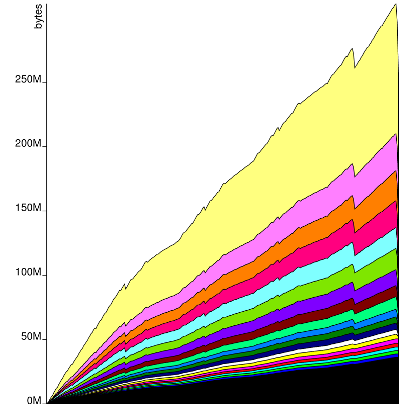
\includegraphics[width=\textwidth]{fig/nodiscard.png}
    \caption{Keeping all results and traces in memory.}
  \end{subfigure}
  \begin{subfigure}{0.49\textwidth}
    \centering
    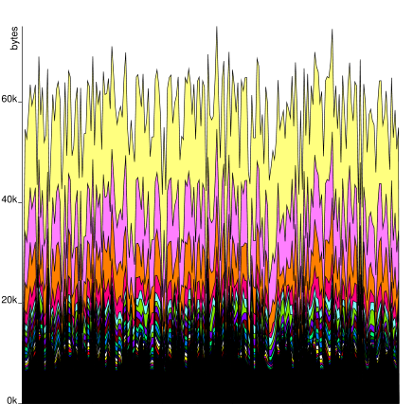
\includegraphics[width=\textwidth]{fig/discard.png}
    \caption{Discarding all traces, just keeping results.}
  \end{subfigure}
  \caption[Heap profiles of a test case for \texttt{MVar} contention.]{Heap profiles of a test case for \texttt{MVar} contention.  Note the dramatic difference: 250M without discarding vs 60k with.  These plots are intended to be viewed with colour.}\label{fig:discard}
\end{figure}

Tweag I/O\footnote{\url{http://www.tweag.io/}}, a research and
development company based in Paris, are using \dejafu{} as part of
their work on a distributed system for the SAGE
project\footnote{\url{http://www.sagestorage.eu/}}, which is
investigating storage systems for future supercomputers.  They cannot
share details of their work for commercial reasons, but one developer
had this to say (emphasis mine):

\begin{displayquote}
  Regarding the test case: we have an implementation of a distributed
  storage cluster, with possibly many nodes and parallel requests.
  The storage system itself is composed of several layers, which can
  be stacked on top of one another.  There is a lot of asynchronicity
  involved.  As per the tests themselves, I am testing parallel
  requests over different objects, etc.

  \emph{I'd like to add that dejafu tests are by far the most reliable
    tests in our suite, in my experience - I am yet to see a
    concurrency bug that they didn't spot, while some other tests
    missed them!} \parencite{tweag2017}
\end{displayquote}

\subsection{Richness of the Abstraction}

As we noted in \Cref{sec:dejafu-whatis-scope}, there are some areas
which we do not currently aim to support with \dejafu{}:

\begin{itemize}
\item Blocking a thread until a file descriptor becomes available, as
  this introduces an additional source of nondeterminism.
\item Throwing an exception to a thread if it becomes deadlocked, as
  we cannot reliably detect deadlock involving only a subset of
  threads without support from the garbage collector.
\item Querying which capability (OS thread) a Haskell thread is
  running on, as this introduces an additional source of
  nondeterminism.
\end{itemize}

These three areas are out of scope because we believe that the desire
for this functionality does not outweigh the implementation cost.  We
will look for a way, if that belief changes.

Introducing additional sources of nondeterminism into an SCT model is
difficult.  Simply introducing additional threads to model the
nondeterminism can cause an explosion of schedules tested, which is
unsatisfactory.  \verb|MonadConc| will always be limited to what
\dejafu{} can reasonably support.

However we can still push back the boundaries of what \dejafu{} supports.
Bound threads, Haskell threads which always run on the same unique OS
thread, were once out of scope as well.  This made it impossible to
use some C libraries with \verb|MonadConc|.  Now we have a prototype
implementation\footnote{\url{https://github.com/barrucadu/dejafu/issues/126}}
which shows promise, and which we intend to release.

\subsection{Writing and Porting Class-polymorphic Code}

\begin{listing}
\centering
\begin{cminted}{haskell}
instance MonadLogger (LoggerT STM) where -- ...
instance MonadLogger (LoggerT IO) where -- ...
\end{cminted}
\caption{Concrete instances for a typeclass-based logging abstraction.}\label{lst:mlogger1}
\end{listing}

We saw in the Par monad example that porting complex code to the
\verb|MonadConc| abstraction is not necessarily a difficult process.
However, this is not always the case.  Recently a user tried to port a
logging abstraction they made to \verb|MonadConc|.  Expressing this
with \verb|MonadConc| and \verb|MonadSTM| is not straightforward, as
constraints do not factor into instance selection.  So the instances
in \Cref{lst:mlogger2} overlap, and are illegal in standard Haskell.

\begin{listing}
\centering
\begin{cminted}{haskell}
instance MonadSTM  m => MonadLogger (LoggerT m) where -- ...
instance MonadConc m => MonadLogger (LoggerT m) where -- ...
\end{cminted}
\caption{Overlapping instances for a typeclass-based logging abstraction.}\label{lst:mlogger2}
\end{listing}

After some work, we introduced new \verb|IsSTM| and \verb|IsConc|
types to disambiguate between the two cases, and ended up with
\Cref{lst:mlogger3}.  The amount of effort required to arrive at this
solution led to the user questioning whether classes like their
\verb|MonadLogger| were even a useful abstraction at
all\footnote{\url{https://www.reddit.com/r/haskell/comments/7b1fbk/do_mtlstyle_effect_classes_really_pull_their/}}!
This is a good topic to think about, but it should not be prompted by
the effort of trying to use \dejafu{}.

\begin{listing}
\centering
\begin{cminted}{haskell}
instance MonadSTM  m => MonadLogger (LoggerT (IsSTM  m)) where -- ...
instance MonadConc m => MonadLogger (LoggerT (IsConc m)) where -- ...
\end{cminted}
\caption{Polymorphic instances for a typeclass-based logging abstraction.}\label{lst:mlogger3}
\end{listing}

So while porting code to the \verb|MonadConc| typeclass is often
simple when dealing with datatype and function definitions, it can be
more complicated when dealing with typeclasses.  It is not clear what
can be done to improve this matter.

\subsection{Library Alternatives}

There are popular Haskell libraries specifically for concurrency.  One
of these is the async library \parencite{async}, part of which we looked at
as a case study~\sref{dejafu-casestudies-async}, for expressing
asynchronous computations.  This library is intended to be a
higher-level and safer way of expressing asynchronous computations
with guaranteed cleanup than using threading, mutable state, and
asynchronous exceptions directly.

Our concurrency library, which provides \verb|MonadConc|, includes an
alternative to async using \verb|MonadConc|.  There is a test suite
using \dejafu{}.  The test suite for async itself just runs most tests
a single time, although one of them is run 1000 times.  Using
\dejafu{} here to automatically seek out interesting schedules is a
much more principled approach then repetition and hope.  Not all
features of async are supported, however.  As we do not currently
support bound threads, functions that use them have been omitted.

This is just one library, and providing an alternative library that
people will have to switch to is far from optimal.  However, until
library authors start to use \dejafu{} and \verb|MonadConc| directly,
such alternatives will be needed to answer the question `Why should I
use this if I cannot use it with anything I use already?'

\subsection{Tool Integration}

There are two popular libraries for unit testing in Haskell,
HUnit \parencite{hunit} and Tasty \parencite{tasty}.  From the perspective of the
user, the libraries are similar, but from the perspective of the
implementer, they have different approaches to integration.  The
hunit-dejafu \parencite{hunit_dejafu} and tasty-dejafu \parencite{tasty_dejafu}
packages provide integration with both.

These packages provide analogues of the \dejafu{} functions, but using
the interface of the testing frameworks, rather than computing and
printing results directly.  The test-framework \parencite{test_framework}
library is also in common use, however it supports integration with
HUnit, and so needs no special support of its own.

The Tasty library is more featureful than HUnit, supporting progress
reporting, giving a message on success as well as failure, and
command-line arguments.  The tasty-dejafu package is similar to the
hunit-dejafu package and does not make use of these additional
features.

\vfill\pagebreak
\section{Summary}

In this chapter we presented \dejafu{}, our tool for testing
concurrent Haskell programs:

\begin{itemize}
\item We provide a typeclass abstraction over concurrency.  Such an
  abstraction allows \verb|IO| to be swapped out and replaced with
  another implementation~\sref{dejafu-monadconc}.

\item We implemented a model of Haskell
  concurrency~\sref{dejafu-execution}, with an empirically derived
  operational semantics~\sref{dejafu-semantics}, so that we can
  simulate the behaviour of GHC.  Our model includes most of the
  Control.Concurrent library module, although some operations are out
  of scope, or have their behaviour changed~\sref{dejafu-whatis-scope}.

\item We use bounded partial-order reduction \parencite{coons2013} with
  relaxed memory \parencite{zhang2015} as the core testing algorithm for
  \dejafu{}, but also support a controlled random scheduling
  approach~\sref{dejafu-testing}.

\item We have not attempted a formal proof of correctness of
  \dejafu{}, but have made an informal correctness argument, noting
  the limits of how correct \dejafu{} can be.  We do have a
  comprehensive test suite, and check what correctness conditions we
  can~\sref{dejafu-correctness}.

\item We have discussed three case studies, all of which involved
  applying \dejafu{} to pre-existing code.  Such code must be modified
  to use the \dejafu{} typeclass abstraction, but we have found this
  to be a straightforward and type-directed process in most
  cases~\sref{dejafu-casestudies}.
\end{itemize}

Although a commonly reported experience amongst Haskell programmers is
that ``if it compiles, it works,'' there are times when it does
\emph{not} work.  Concurrency is a particularly difficult area to get
right, as everyone who has had to move outside the realm of guaranteed
determinism will know.  By developing \dejafu{}, we hope that
concurrency in Haskell will become a little easier to get right.

\paragraph{Context}
\dejafu{} does not stand alone, it is related to our other
contributions:

\begin{itemize}
\item \Cref{chp:algorithms} discusses a new random scheduling
  algorithm for incomplete concurrency testing.  The chapter does not
  directly build on \dejafu{}, but \dejafu{} implements the algorithm.
\item \Cref{chp:coco} discusses a new property-discovery tool for
  functions operating on mutable state.  The tool directly builds on
  \dejafu{} in two ways: (1) to discover these properties, and (2) by
  providing an interface for \dejafu{} to check them.
\end{itemize}
